\documentclass[seriffont, cmap=Beijing, 10pt]{zz}

\newcommand\hmmax{0}
\newcommand\bmmax{0}

\usepackage[utf8]{inputenc}
\usepackage[T1]{fontenc}
%\usepackage{fouriernc}
\usepackage{amsmath, amssymb, bm, mathtools}
\usepackage{animate}
\usepackage{graphicx}

\usepackage{tikz}
\usetikzlibrary{fadings}
\usetikzlibrary{patterns}
\usetikzlibrary{shadows.blur}
\usetikzlibrary{shapes}

\title{Lectio Praecursoria}
\subtitle{State-Space Deep Gaussian Processes with Applications}

\date[10 December 2021]{10 December 2021}
\institute{Aalto University}

\author[Zheng Zhao]{Zheng Zhao}

\setbeamercovered{transparent}
\setbeamertemplate{section in toc}[circle]

% Change toc item spacing
% https://tex.stackexchange.com/questions/170268/separation-space-between-tableofcontents-items-in-beamer
\usepackage{etoolbox}
\makeatletter
\patchcmd{\beamer@sectionintoc}
{\vfill}
{\vskip2.\itemsep}
{}
{}
\makeatother  

% Footnote without numbering
% https://tex.stackexchange.com/questions/30720/footnote-without-a-marker
\newcommand\blfootnote[1]{%
	\begingroup
	\renewcommand\thefootnote{}\footnote{\scriptsize#1}%
	\addtocounter{footnote}{-1}%
	\endgroup
}

%!TEX root = dissertation.tex
% Generic macro definitions for a number of math operations.
%
% To use this macro you need packages: amsmath, amssymb, bm, mathtools
%
% Zheng Zhao @ 2019
% zz@zabemon.com
%
% License: Creativice Commons Attribution 4.0 International (CC BY 4.0)
%

% Adaptive bold math font command
\newcommand{\cu}[1]{
	\ifcat\noexpand#1\relax
	\bm{#1}
	\else
	\mathbf{#1}
	\fi
}

\newcommand{\tash}[2]{\frac{\partial #1}{\partial #2}}
\newcommand{\tashh}[3]{\frac{\partial^2 #1}{\partial #2 \, \partial #3}}

% Slightly smaller spacing than a pure mathop
\newcommand{\diff}{\mathop{}\!\mathrm{d}}

% Complex
\newcommand{\imag}{\mathrm{i}}

% Exponential
\newcommand{\expp}{\mathrm{e}}

% \mid used in condition in probability e.g., E[x \mid y]
\newcommand{\cond}{{\;|\;}}
\newcommand{\condbig}{{\;\big|\;}}
\newcommand{\condBig}{{\;\Big|\;}}
\newcommand{\condbigg}{{\;\bigg|\;}}
\newcommand{\condBigg}{{\;\Bigg|\;}}

\let\sup\relax
\let\inf\relax
\let\lim\relax
\DeclareMathOperator*{\argmin}{arg\,min\,}  % Argmin
\DeclareMathOperator*{\argmax}{arg\,max\,}  % Argmax
\DeclareMathOperator*{\sup}{sup\,}  % sup better spacing
\DeclareMathOperator*{\inf}{inf\,}  % inf
\DeclareMathOperator*{\lim}{lim\,}  % inf

\newcommand{\sgn}{\operatorname{sgn}}           % sign function

\newcommand{\expecsym}{\operatorname{\mathbb{E}}}     % Expec
\newcommand{\covsym}{\operatorname{Cov}}     % Covariance
\newcommand{\varrsym}{\operatorname{Var}}     % Variance
\newcommand{\diagsym}{\operatorname{diag}}     % Diagonal matrix
\newcommand{\tracesym}{\operatorname{tr}}           % Trace

% Two problems for E, Cov, Var etc. with brackets
% 1. \operatorname does not give space for bracket, thus we need to manually add \, after E. If \left\right is used then no need to add space.
% 2. \left\right does not give correct vertical spacing. The brackets will be shifted down slightly.
% Solution is to use \left\right when it is inevitable.
% Use \expec when you do not want auto-height
% Use \expec* when you want auto-height
% Use \expecsym when you want to fully define the behaviour, which only gives the E symbol wihout brackets. 
\let\expec\relax
\let\cov\relax
\let\varr\relax
\let\diag\relax
\let\trace\relax

\makeatletter
% E [ ]
\newcommand{\expec}{\@ifstar{\@expecauto}{\@expecnoauto}}
\newcommand{\@expecauto}[1]{\expecsym \left[ #1 \right]}
\newcommand{\@expecnoauto}[1]{\expecsym [#1]}
\newcommand{\expecbig}[1]{\expecsym \bigl[ #1 \bigr]}
\newcommand{\expecBig}[1]{\expecsym \Bigl[ #1 \Bigr]}
\newcommand{\expecbigg}[1]{\expecsym \biggl[ #1 \biggr]}
\newcommand{\expecBigg}[1]{\expecsym \Biggl[ #1 \Biggr]}


% Cov [ ]
\newcommand{\cov}{\@ifstar{\@covauto}{\@covnoauto}}
\newcommand{\@covauto}[1]{\covsym \left[ #1 \right]}
\newcommand{\@covnoauto}[1]{\covsym [#1]}
\newcommand{\covbig}[1]{\covsym \bigl[ #1 \bigr]}
\newcommand{\covBig}[1]{\covsym \Bigl[ #1 \Bigr]}
\newcommand{\covbigg}[1]{\covsym \biggl[ #1 \biggr]}
\newcommand{\covBigg}[1]{\covsym \Biggl[ #1 \Biggr]}

% Var [ ]
\newcommand{\varr}{\@ifstar{\@varrauto}{\@varrnoauto}}
\newcommand{\@varrauto}[1]{\varrsym \left[ #1 \right]}
\newcommand{\@varrnoauto}[1]{\varrsym [#1]}
\newcommand{\varrbig}[1]{\varrsym \bigl[ #1 \bigr]}
\newcommand{\varrBig}[1]{\varrsym \Bigl[ #1 \Bigr]}
\newcommand{\varrbigg}[1]{\varrsym \biggl[ #1 \biggr]}
\newcommand{\varrBigg}[1]{\varrsym \Biggl[ #1 \Biggr]}

% Diag ( )
\newcommand{\diag}{\@ifstar{\@diagauto}{\@diagnoauto}}
\newcommand{\@diagauto}[1]{\diagsym \left( #1 \right)}
\newcommand{\@diagnoauto}[1]{\diagsym (#1)}
\newcommand{\diagbig}[1]{\diagsym \bigl( #1 \bigr)}
\newcommand{\diagBig}[1]{\diagsym \Bigl( #1 \Bigr)}
\newcommand{\diagbigg}[1]{\diagsym \biggl( #1 \biggr)}
\newcommand{\diagBigg}[1]{\diagsym \Biggl( #1 \Biggr)}

% tr ( )
\newcommand{\trace}{\@ifstar{\@traceauto}{\@tracenoauto}}
\newcommand{\@traceauto}[1]{\tracesym \left( #1 \right)}
\newcommand{\@tracenoauto}[1]{\tracesym (#1)}
\newcommand{\tracebig}[1]{\tracesym \bigl( #1 \bigr)}
\newcommand{\traceBig}[1]{\tracesym \Bigl( #1 \Bigr)}
\newcommand{\tracebigg}[1]{\tracesym \biggl( #1 \biggr)}
\newcommand{\traceBigg}[1]{\tracesym \Biggl( #1 \Biggr)}
\makeatother

\newcommand{\A}{\mathcal{A}}           % Generator
\newcommand{\Am}{\overline{\mathcal{A}}}           % Generator

% Transpose symbol using (DIN) EN ISO 80000-2:2013 standard
\newcommand*{\trans}{{\mkern-1.5mu\mathsf{T}}}

\newcommand*{\T}{\mathbb{T}} % Set of temporal varialbes
\newcommand*{\R}{\mathbb{R}} % Set of real numbers
\newcommand*{\Q}{\mathbb{Q}} % Set of rational numbers
\newcommand*{\N}{\mathbb{N}} % Set of natural numbers
\newcommand*{\Z}{\mathbb{Z}} % Set of integers

\newcommand*{\BB}{\mathcal{B}} % Borel sigma-algebra
\newcommand*{\FF}{\mathcal{F}} % Sigma-algebra
\newcommand*{\PP}{\mathbb{P}} % Probability measure
\newcommand*{\GP}{\mathrm{GP}} % GP

\newcommand{\mineig}{\lambda_{\mathrm{min}}}
\newcommand{\maxeig}{\lambda_{\mathrm{max}}}

% Norm and inner product
%% use \norm* to enable auto-height

%% Some notes on these paired delimiters:
%% It is argued that there should be no space between operator and delimiter, but this might not be suitable in some cases. Indeed log(x) should have no space between log and (, but log |x| with a mathop{} spacing looks absolutely much prettier than log|x| because here |x| is an argument. Think, shouldn't it be log(|x|) in full expansion, and we ignored () with spacing?
%% See discussion in https://tex.stackexchange.com/questions/461806/missing-space-with-declarepaireddelimiter
%
\let\norm\relax
\DeclarePairedDelimiter{\normbracket}{\lVert}{\rVert}
\newcommand{\norm}{\normbracket}
\newcommand{\normbig}[1]{\big \lVert #1 \big \rVert}
\newcommand{\normBig}[1]{\Big \lVert #1 \Big\rVert}
\newcommand{\normbigg}[1]{\bigg \lVert #1 \bigg\rVert}
\newcommand{\normBigg}[1]{\Bigg \lVert #1 \Bigg\rVert}
%\makeatletter
%\newcommand{\norm}{\@ifstar{\@normnoauto}{\@normauto}}
%\newcommand{\@normauto}[1]{\left\lVert#1\right\rVert}
%\newcommand{\@normnoauto}[1]{\lVert#1\rVert}
%\makeatother

\let\innerp\relax
\DeclarePairedDelimiter{\innerpbracket}{\langle}{\rangle}
\newcommand{\innerp}{\innerpbracket}
%\makeatletter
%\newcommand{\innerp}{\@ifstar{\@inpnoautp}{\@inpauto}}
%\newcommand{\@inpauto}[2]{\left\langle#1, #2\right\rangle}
%\newcommand{\@inpnoautp}[2]{\left#1, #2\rangle}
%\makeatother

\let\abs\relax
\DeclarePairedDelimiter{\absbracket}{\lvert}{\rvert}
\newcommand{\abs}{\absbracket}
\newcommand{\absbig}[1]{\big \lvert #1 \big \rvert}
\newcommand{\absBig}[1]{\Big \lvert #1 \Big\rvert}
\newcommand{\absbigg}[1]{\bigg \lvert #1 \bigg\rvert}
\newcommand{\absBigg}[1]{\Bigg \lvert #1 \Bigg\rvert}
%\makeatletter
%\newcommand{\abs}{\@ifstar{\@absnoauto}{\@absauto}}
%\newcommand{\@absauto}[1]{\left\lvert#1\right\rvert}
%\newcommand{\@absnoauto}[1]{\lvert#1\rvert}
%\makeatother

% Some functions
\newcommand{\mBesselsec}{\operatorname{K}_\nu}
\newcommand{\jacob}{\operatorname{J}}
\newcommand{\hessian}{\operatorname{H}}

% Literals
\def\matern{Mat\'{e}rn }

% Theorem envs
% Dummy env for those sharing the same numbering system.
% If you would like to customise your environment numbering, you can define a command e.g., \thmnumcounter{section} in your main tex.
% If \thmnumcounter is undefined, it is assumed that you will deal with defining theorem lemma etc by yourself.
\makeatletter
\@ifundefined{thmenvcounter}{}
{%
	\newtheorem{envcounter}{EnvcounterDummy}[\thmenvcounter]
	\newtheorem{theorem}[envcounter]{Theorem}
	\newtheorem{proposition}[envcounter]{Proposition}
	\newtheorem{lemma}[envcounter]{Lemma}
	\newtheorem{corollary}[envcounter]{Corollary}
	\newtheorem{remark}[envcounter]{Remark}
	\newtheorem{example}[envcounter]{Example}
	\newtheorem{definition}[envcounter]{Definition}
	\newtheorem{algorithm}[envcounter]{Algorithm}
	\newtheorem{assumption}[envcounter]{Assumption}
}
\makeatother


\begin{document}

\titlepage

\begin{frame}{The dissertation}
	\noindent
	\begin{minipage}{.48\textwidth}
		\begin{figure}
			\centering
			\fbox{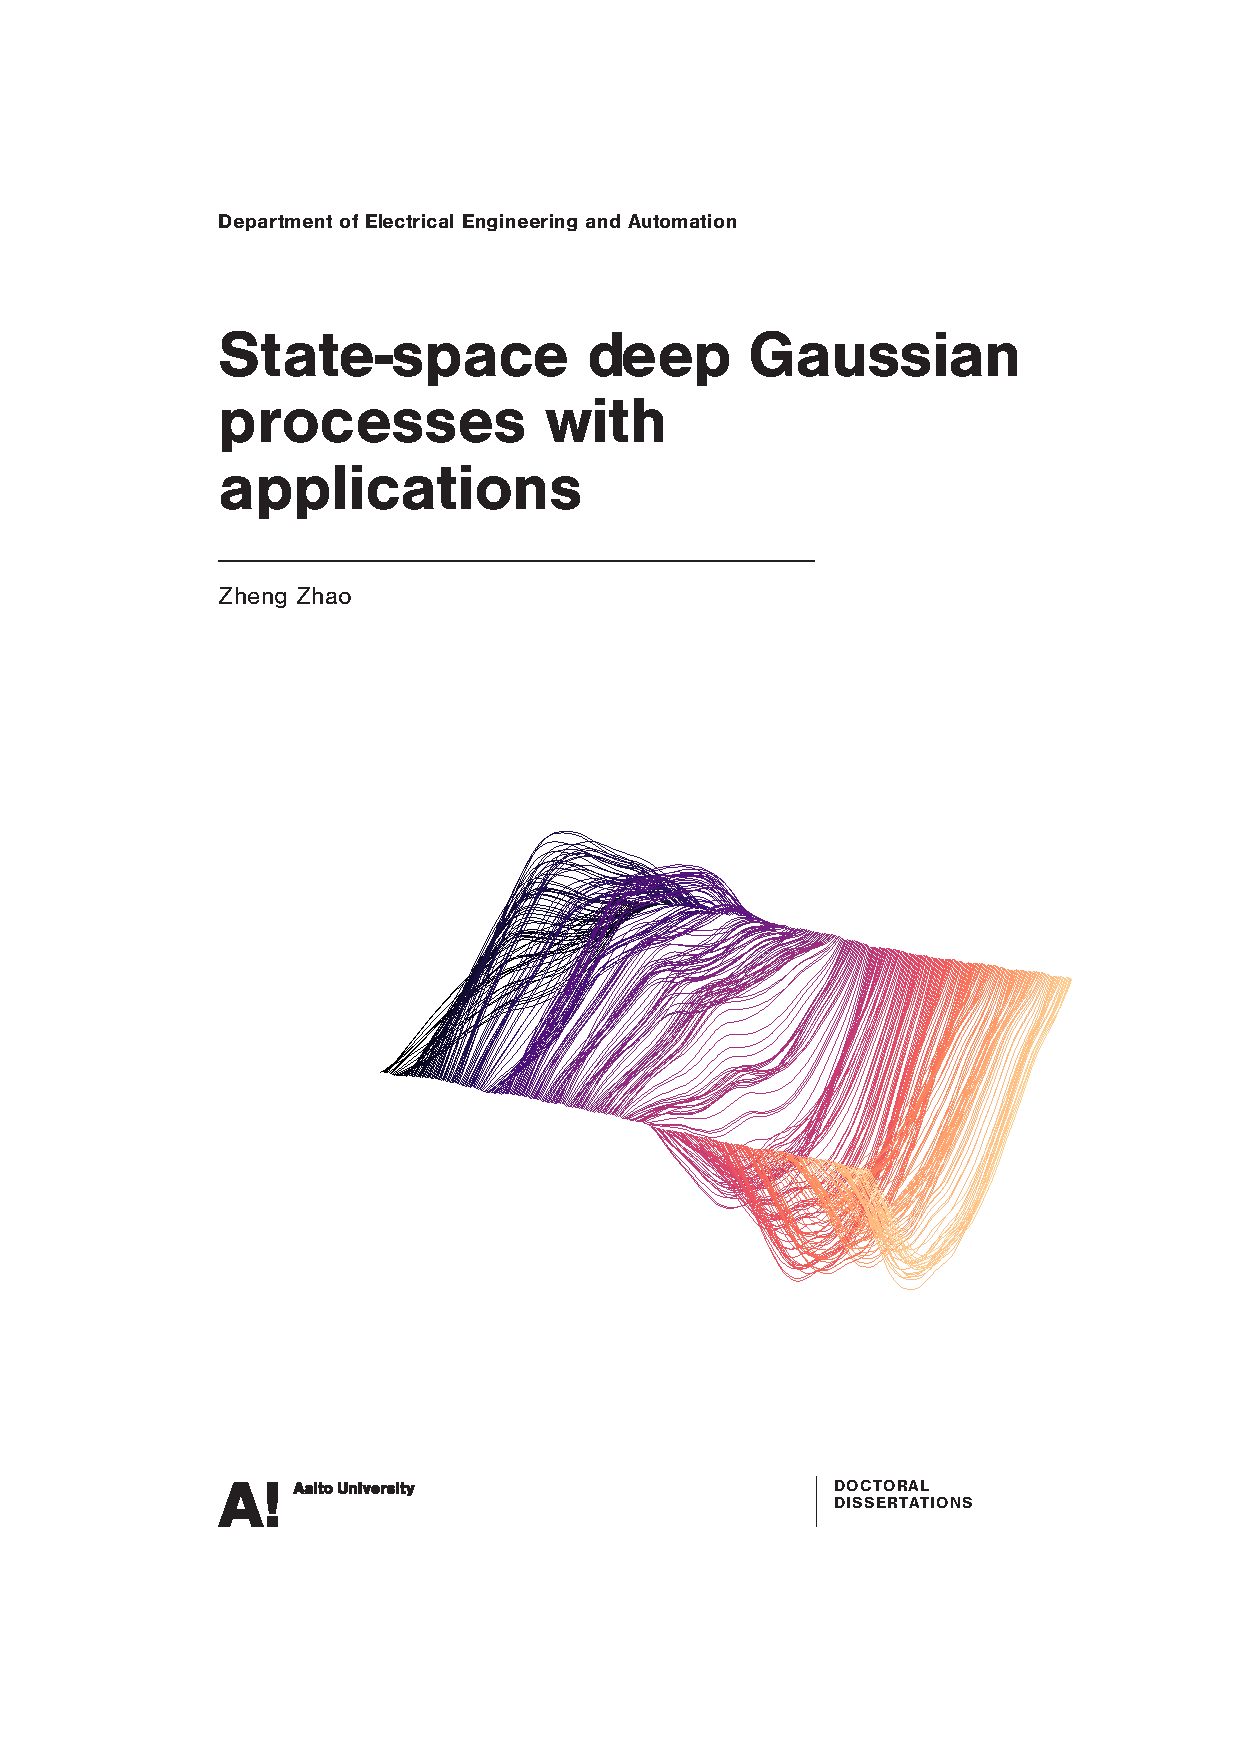
\includegraphics[trim={2cm 2cm 2cm 2cm},width=.8\linewidth,clip]{../thesis_latex/title-pages/title-pages}}
		\end{figure}
	\end{minipage}
	\hfill
	\begin{minipage}{.48\textwidth}
		\begin{block}{}
			Available online:\\ \url{https://github.com/zgbkdlm/dissertation}\\
			or scan the QR code
		\end{block}
		\begin{block}{}
			\begin{figure}
				\centering
				
\includegraphics[width=.5\linewidth]{figs/qr-code-thesis}
			\end{figure}
		\end{block}
		\begin{block}{}
			Companion codes in Python and Matlab are also in $^\wedge$
		\end{block}
	\end{minipage}
\end{frame}

\begin{frame}{Contents}
	This dissertation mainly consists of:
	\begin{block}{}
		\tableofcontents
	\end{block}
\end{frame}

\section{Continuous-discrete filtering and smoothing with Taylor moment expansion}
\begin{frame}{Contents}
	\begin{block}{}
		\tableofcontents[currentsection]
	\end{block}
\end{frame}

\begin{frame}{Stochastic filtering}
	\begin{block}{}
		Consider a system
		%
		\begin{equation}
			\begin{split}
				\diff X(t) &= a(X(t)) \diff t + b(X(t)) \diff W(t), \quad X(t_0) = X_0,\\
				Y_k &= h(X(t_k)) + \xi_k, \quad \xi_k \sim \mathrm{N}(0, \Xi_k),
			\end{split}
		\end{equation}
		%
		and a set of data $y_{1:T} = \lbrace y_1, y_2,\ldots, y_T \rbrace$. The goals are to estimate
		\begin{itemize}
			\item the (marginal) \alert{filtering} distributions
			%
			\begin{equation}
				p(x_k \cond y_{1:k}), \quad \text{for }k=1,2,\ldots,
			\end{equation}
			%
			\item and the (marginal) \alert{smoothing} distributions
			%
			\begin{equation}
				p(x_k \cond y_{1:T}), \quad \text{for }k=1,2,\ldots,T,
			\end{equation}
			%
		\end{itemize}
	\end{block}
	\blfootnote{$p(x \cond y)$ abbreviates $p_{X \cond Y}(x \cond y)$.}
\end{frame}

\begin{frame}{Stochastic filtering}
	\begin{block}{}
		\begin{figure}
			\centering
			\animategraphics[autoplay, loop, width=.49\linewidth]{10}{figs/animes/filter-}{0}{99}
			\animategraphics[autoplay, loop, width=.49\linewidth]{10}{figs/animes/smoother-}{0}{99}
			\caption{Filtering (left) and smoothing (right).}
%			dummy image
		\end{figure}
	\end{block}
\end{frame}

\begin{frame}{Stochastic filtering}
	\begin{block}{}
		Solving the \alert{filtering} and \alert{smoothing} problems usually involves computing
		%
		\begin{equation}
			\expec{\phi(X(t)) \cond X(s)}
		\end{equation}
		%
		for $t\geq s \in\T$ and some \alert{target function $\phi$}.
	\end{block}
	\begin{block}{}
		For instance, in \alert{Gaussian} approximate filtering and smoothing, we choose $\phi^\mathrm{I}(x)\coloneqq x$ and $\phi^\mathrm{II}(x)\coloneqq x \, x^\trans$ in order to approximate
		%
		\begin{equation}
			\begin{split}
				p(x_k \cond y_{1:k}) &\approx \mathrm{N}\big(x_k \cond m^f_k, P^f_k\big), \\
				p(x_k \cond y_{1:T}) &\approx \mathrm{N}\big(x_k \cond m^s_k, P^s_k\big).
			\end{split}
		\end{equation}
		%
	\end{block}
\end{frame}

\begin{frame}{Stochastic filtering}
	\begin{block}{}
		Thanks to D. Florens-Zmirou and D. Dacunha-Castelle, for any $\phi\in \mathcal{C}(\R^{2\,(M+1)};\R)$, it is possible to
		%
		\begin{equation}
			\expec{\phi(X(t)) \cond X(s)} = \sum^M_{r=0} \A^r\phi(X(s))\,\Delta t^r + R_{M, \phi}(X(s), \Delta t),
		\end{equation}
		%
		where
		%
		\begin{equation}
			\begin{split}
				\A\phi(x) &\coloneqq (\nabla_x\phi(x))^\trans \, a(x) + \frac{1}{2} \, \tracebig{\Gamma(x) \, \hessian_x\phi(x)},\\
				\Gamma(x) &\coloneqq b(x) \, b(x)^\trans.
			\end{split}
		\end{equation}
		%
	\end{block}
	\begin{block}{}
		We call this \alert{Taylor moment expansion (TME)}, detailed in Section 3.3.
	\end{block}
\end{frame}

\begin{frame}{Stochastic filtering}
	\begin{block}{}
		However, the TME approximation to the \alert{covariance} $\cov{X(t) \cond X(s)}$ might not be \alert{positive definite}. Detailed in \alert{Theorem~3.5}.
	\end{block}
	\begin{block}{}
		This problem can be numerically addressed by:
		\begin{itemize}
			\item Choose small \alert{time interval} $t-s$.
			\item Increase the expansion \alert{order} $M$ if the SDE coefficients are regular enough.
			\item Tune SDE coefficients so that it's positive definite for all $t-s\in\R_{>0}$ (see \alert{Corollary 3.6}).
			\item Tune SDE coefficients so that it's positive definite for all $X(s)\in\R^d$ (see \alert{Lemma 3.8}).
		\end{itemize}
	\end{block}
\end{frame}

\begin{frame}{Stochastic filtering}
	\begin{block}{}
		\begin{example}
			\begin{equation}
				\begin{split}
					\diff X^1(t) &= \big( \log(1+\exp(X^1(t))) + \kappa\,X^2(t) \big)\diff t + \diff W_1(t),\\
					\diff X^2(t) &= \big( \log(1+\exp(X^2(t))) + \kappa\,X^1(t) \big)\diff t + \diff W_2(t),\\
					X^1(t_0)&=X^2(t_0)=0,
				\end{split}
			\end{equation}
			where $\kappa\in\R$ is a \alert{tunable} parameter. By applying \alert{Corollary 3.6}, the TME-2 covariance approximation to this SDE is positive definite for \alert{all} $t-t_0\in\R_{>0}$, if \alert{$\abs{\kappa}\leq0.5$}.
		\end{example}
	\end{block}
\end{frame}

%\begin{frame}{Stochastic filtering}
%	\begin{block}{}
%		\begin{figure}
%			\centering
%			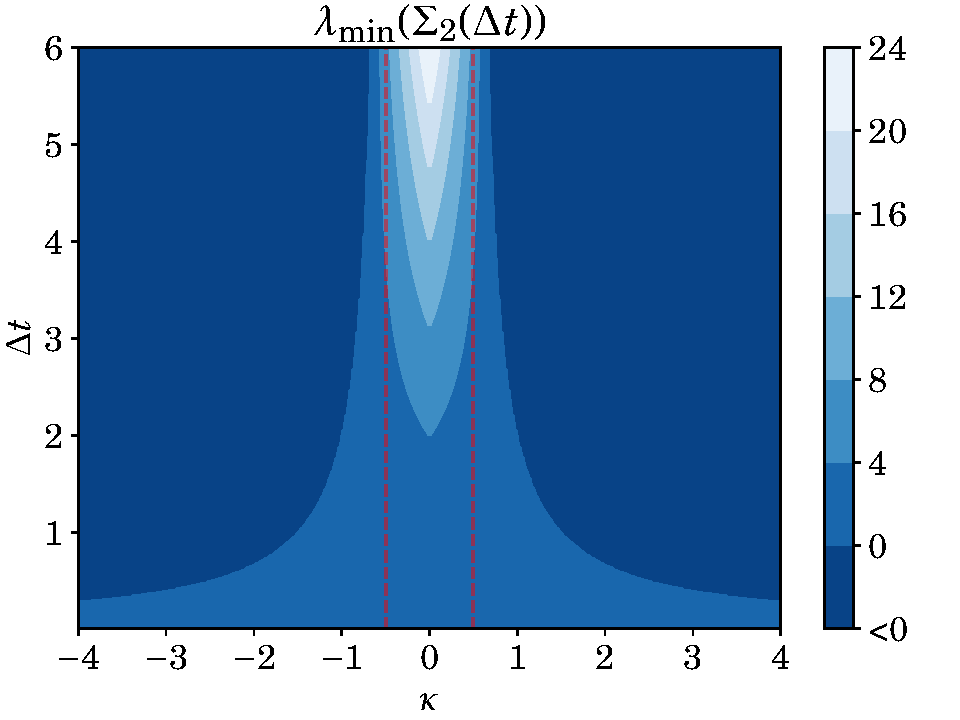
\includegraphics[width=.7\linewidth]{../thesis_latex/figs/tme-softplus-mineigs}
%			\caption{The minimum eigenvalues of TME-2 approximated $\cov{X(t) \cond X(t_0)}$ (denote $\Sigma_2$) w.r.t. $\Delta t=t-t_0$ and $\kappa$.}
%		\end{figure}
%	\end{block}
%\end{frame}

\begin{frame}{Stochastic filtering}
	\begin{block}{}
		\alert{Section 3.6} details how to run Gaussian filters and smoothers with the TME method.
	\end{block}
	\begin{block}{}
		Under a few assumptions on the system, the TME Gaussian filters and smoothers are \alert{stable} in the sense that (\alert{Theorem 3.17})
		%
		\begin{equation}
			\expecBig{\normbig{X_k - m^f_k}_2^2} \leq (c^f_1)^k \, \trace{P_0} + c^f_2, \quad k=1,2,\ldots
		\end{equation}
		%
		and 
		\begin{equation}
			\begin{split}
				\expecBig{\normbig{X_k - m^s_k}_2^2} &\leq c^f_0(k) + (c^s_1)^{T-k} \, c_2 + c_3, \quad,\\
				k&=1,2,\ldots,T, \quad T=1,2,\ldots,
			\end{split}
		\end{equation}
		where $c^f_1<1$, $c^s_1<1$, and $c^f_0(k)$ depends on $\expec{\norm{X_k - m^f_k}_2^2}$ \alert{only}. 
	\end{block}
\end{frame}

\begin{frame}{Stochastic filtering}
	\begin{figure}
		\centering
		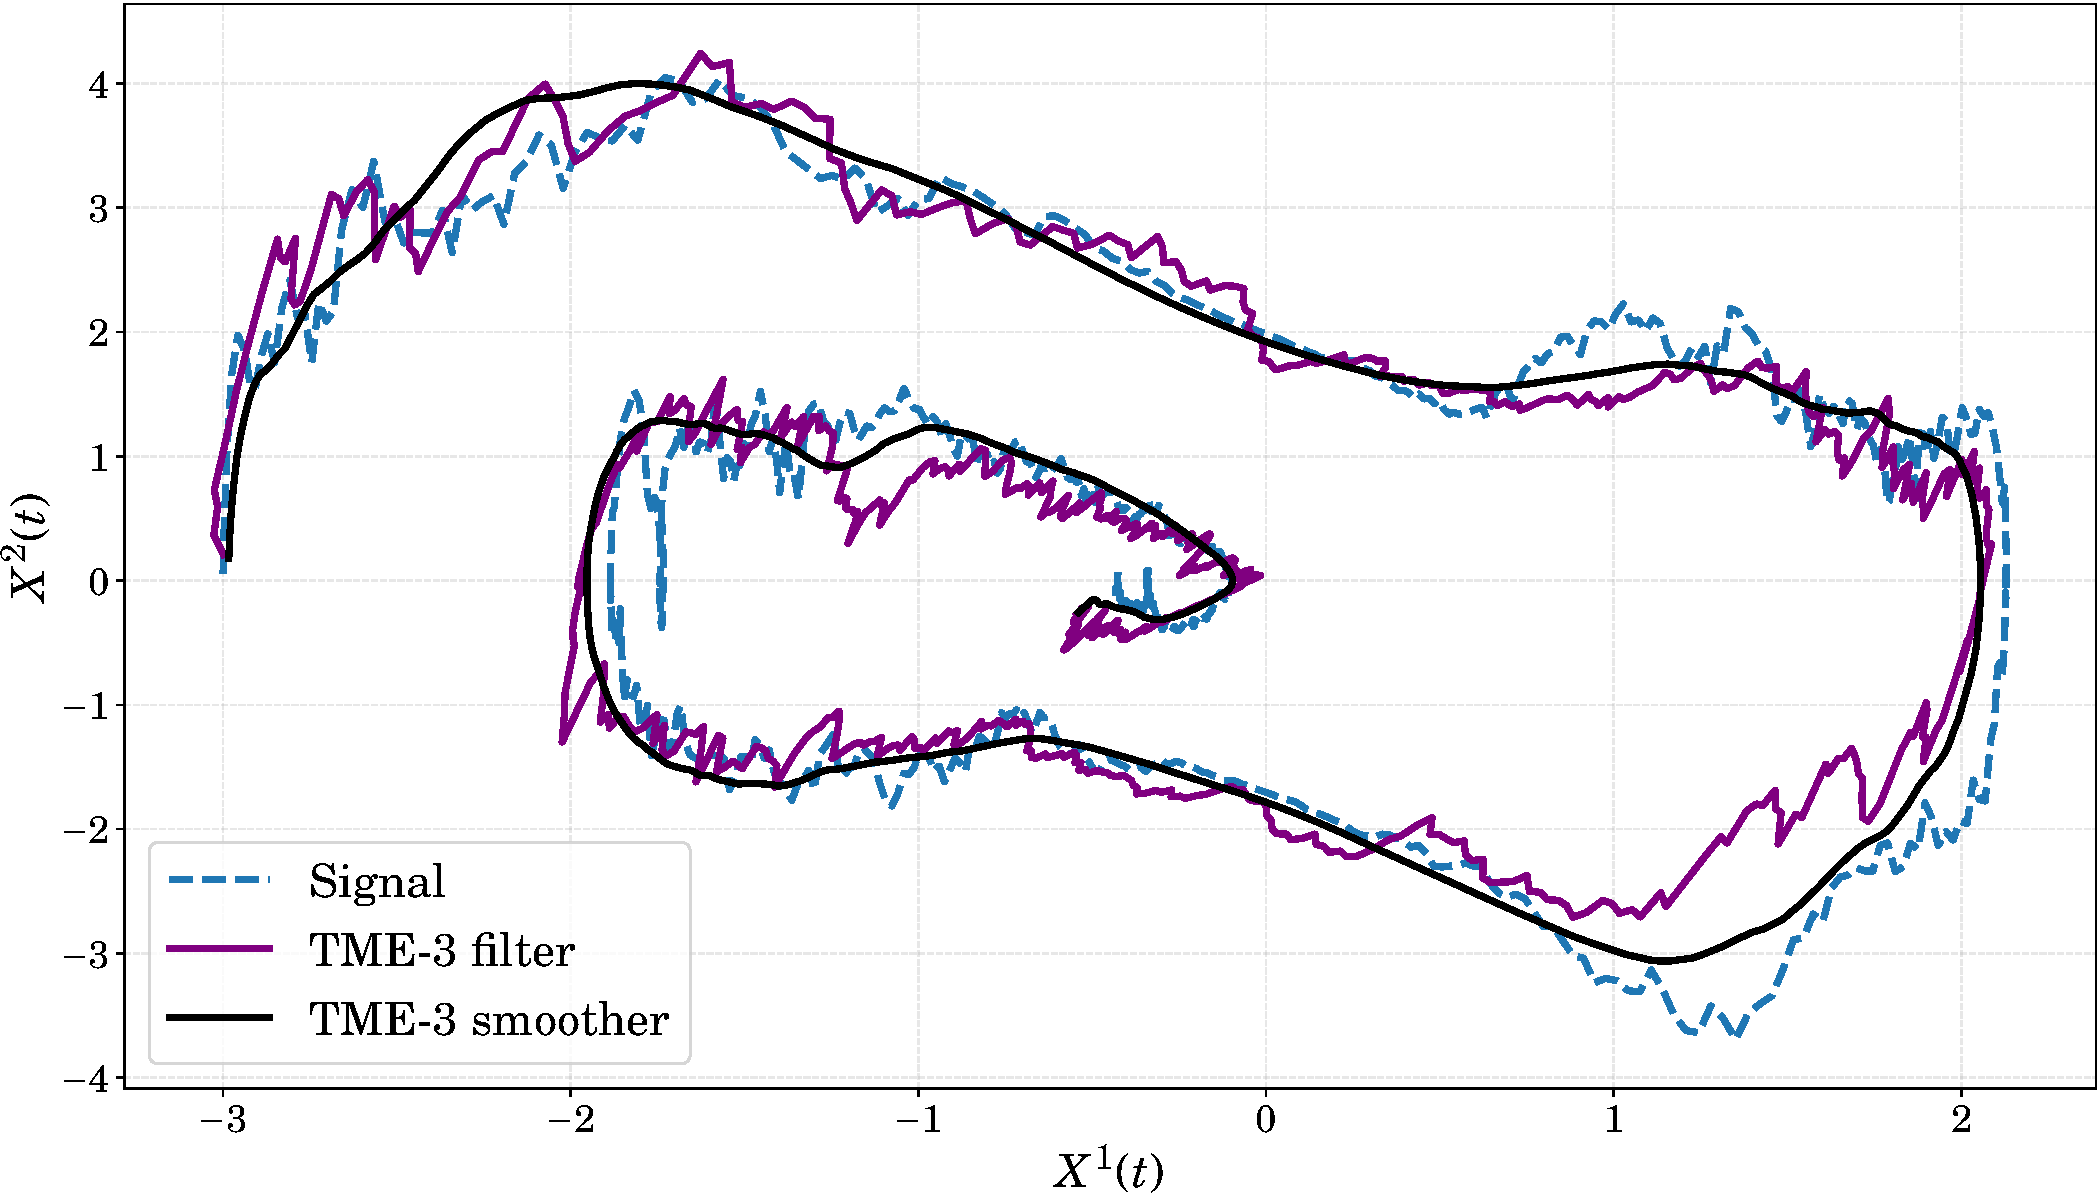
\includegraphics[width=.6\linewidth]{../thesis_latex/figs/tme-duffing-filter-smoother}\\
		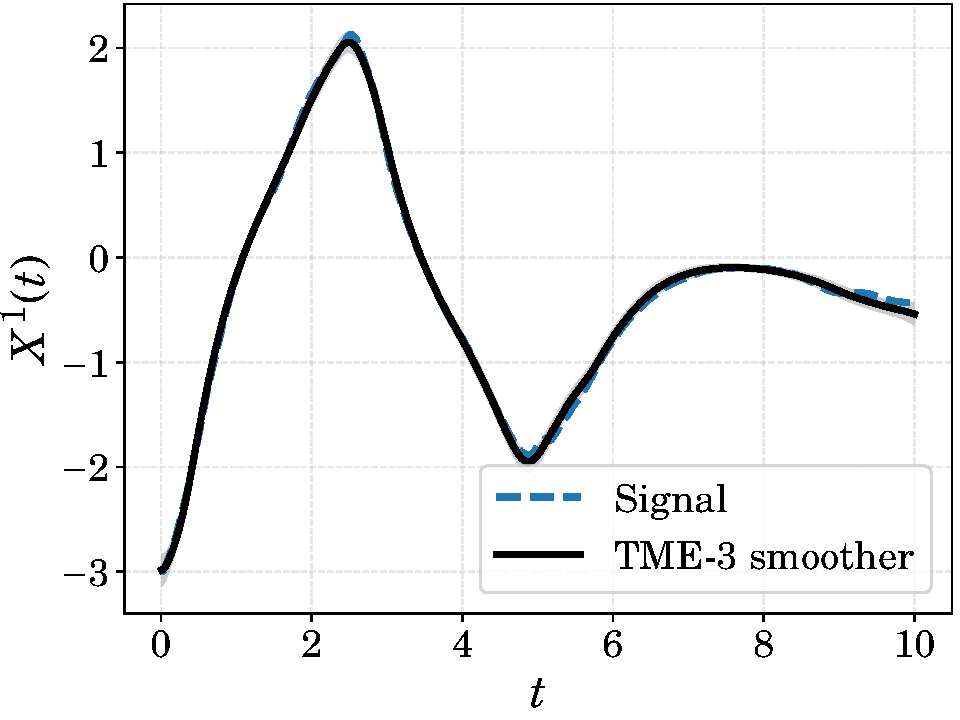
\includegraphics[width=.4\linewidth]{../thesis_latex/figs/tme-duffing-smoother-x1}
		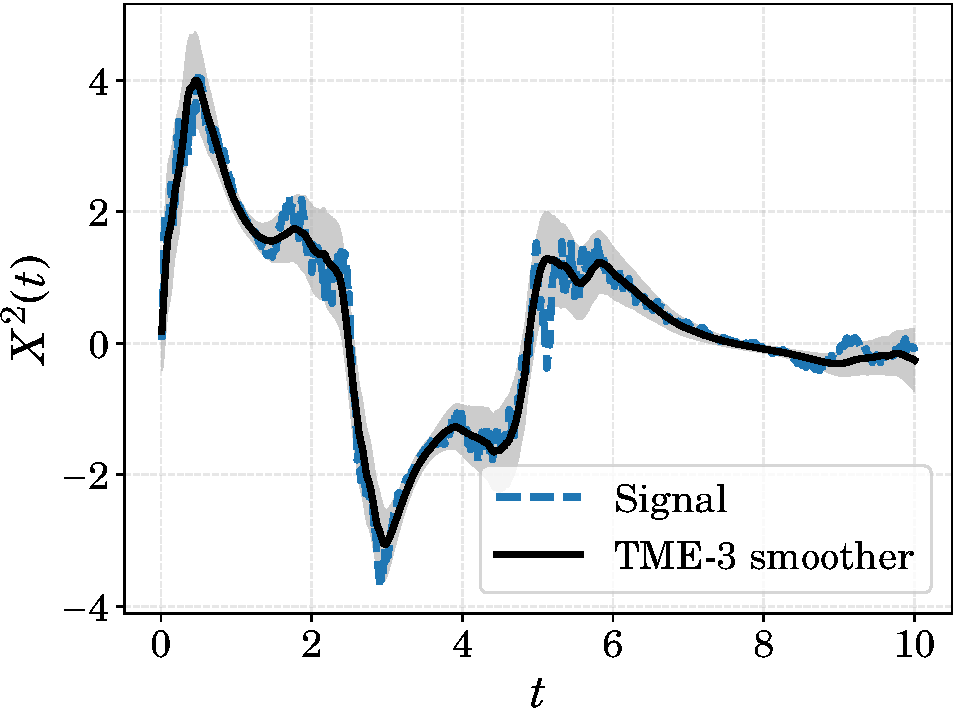
\includegraphics[width=.4\linewidth]{../thesis_latex/figs/tme-duffing-smoother-x2}
		\caption{TME on Duffing-van der Pol (\alert{Example 3.19}).}
	\end{figure}
\end{frame}

\section{State-space deep Gaussian processes}
\begin{frame}{Contents}
	\begin{block}{}
		\tableofcontents[currentsection]
	\end{block}
\end{frame}

%\begin{frame}{Gaussian processes}
%	\begin{block}{}
%		$U\colon\T\to\R^d$ is said to be a \alert{Gaussian process (GP)}, if for every $t_1<t_2<\cdots<t_k\in\T$, the random variables $U(t_1), U(t_2), \ldots, U(t_k)$ are Normal distributed. Denoted by (for simplicity, zero mean)
%		%
%		\begin{equation}
%			U(t) \sim \GP\big( 0, C(t,t'; \theta) \big),
%		\end{equation}
%		%
%	\end{block}
%	\begin{block}{}
%		A class of \alert{Markov} GPs are governed by linear SDEs of the form:
%		%
%		\begin{equation}
%			\diff U(t) = A(t; \theta) \, U(t) \diff t + B(t; \theta) \diff W(t), \quad U_0\sim \mathrm{N}(0, P_0(\theta)).
%		\end{equation}
%		%
%	\end{block}
%\end{frame}

\begin{frame}{Gaussian processes}
		Denote GP by
		%
		\begin{equation}
			U(t) \sim \GP\big( 0, C(t,t'; \theta) \big),
		\end{equation}
		%
		and a class of \alert{Markov} GPs by \alert{linear SDEs} of the form
		%
		\begin{equation}
			\diff U(t) = A(t; \theta) \, U(t) \diff t + B(t; \theta) \diff W(t), \quad U_0\sim \mathrm{N}(0, P_0(\theta)).
		\end{equation}
		%
		\begin{figure}
			\centering
			\includegraphics[width=.4\linewidth]{figs/gp-sample-m12}
			\includegraphics[width=.4\linewidth]{figs/gp-sample-m32}
			\caption{Samples drawn from two \alert{stationary} GPs.}
		\end{figure}
\end{frame}

\begin{frame}{SS-DGPs}
		To make \alert{non-stationary} ``GPs'', one can let their parameters $\theta$ be processes of $t$, and the parameters of $\theta$ be processes of $t$ again, and so forth following this analogy...
		This leads to \alert{a} class of \alert{deep GPs (DGPs)}, see Introduction and \alert{Section 4.3}.
	\begin{figure}[t!]
		\centering
		\resizebox{.35\linewidth}{!}{%
			\tikzset{every picture/.style={line width=0.75pt}} %set default line width to 0.75pt        

\begin{tikzpicture}[x=0.6pt,y=0.6pt,yscale=-1,xscale=1]
%uncomment if require: \path (0,300); %set diagram left start at 0, and has height of 300

%Shape: Circle [id:dp821654118938725] 
\draw  [line width=1.5]  (200,30) .. controls (200,18.95) and (208.95,10) .. (220,10) .. controls (231.05,10) and (240,18.95) .. (240,30) .. controls (240,41.05) and (231.05,50) .. (220,50) .. controls (208.95,50) and (200,41.05) .. (200,30) -- cycle ;
%Shape: Circle [id:dp7532382575897598] 
\draw  [line width=1.5]  (150,100) .. controls (150,88.95) and (158.95,80) .. (170,80) .. controls (181.05,80) and (190,88.95) .. (190,100) .. controls (190,111.05) and (181.05,120) .. (170,120) .. controls (158.95,120) and (150,111.05) .. (150,100) -- cycle ;
%Shape: Circle [id:dp5902978501813476] 
\draw  [line width=1.5]  (250,100) .. controls (250,88.95) and (258.95,80) .. (270,80) .. controls (281.05,80) and (290,88.95) .. (290,100) .. controls (290,111.05) and (281.05,120) .. (270,120) .. controls (258.95,120) and (250,111.05) .. (250,100) -- cycle ;
%Straight Lines [id:da9016881764549007] 
\draw [line width=1.5]    (207.17,52.83) -- (180,80) ;
\draw [shift={(210,50)}, rotate = 135] [fill={rgb, 255:red, 0; green, 0; blue, 0 }  ][line width=0.08]  [draw opacity=0] (13.4,-6.43) -- (0,0) -- (13.4,6.44) -- (8.9,0) -- cycle    ;
%Straight Lines [id:da026586992089503658] 
\draw [line width=1.5]    (232.83,52.83) -- (260,80) ;
\draw [shift={(230,50)}, rotate = 45] [fill={rgb, 255:red, 0; green, 0; blue, 0 }  ][line width=0.08]  [draw opacity=0] (13.4,-6.43) -- (0,0) -- (13.4,6.44) -- (8.9,0) -- cycle    ;
%Shape: Circle [id:dp7932559631044391] 
\draw  [line width=1.5]  (100,170) .. controls (100,158.95) and (108.95,150) .. (120,150) .. controls (131.05,150) and (140,158.95) .. (140,170) .. controls (140,181.05) and (131.05,190) .. (120,190) .. controls (108.95,190) and (100,181.05) .. (100,170) -- cycle ;
%Shape: Circle [id:dp8827895580667542] 
\draw  [line width=1.5]  (170,170) .. controls (170,158.95) and (178.95,150) .. (190,150) .. controls (201.05,150) and (210,158.95) .. (210,170) .. controls (210,181.05) and (201.05,190) .. (190,190) .. controls (178.95,190) and (170,181.05) .. (170,170) -- cycle ;
%Shape: Circle [id:dp1311962702995253] 
\draw  [line width=1.5]  (230,170) .. controls (230,158.95) and (238.95,150) .. (250,150) .. controls (261.05,150) and (270,158.95) .. (270,170) .. controls (270,181.05) and (261.05,190) .. (250,190) .. controls (238.95,190) and (230,181.05) .. (230,170) -- cycle ;
%Shape: Circle [id:dp055039676738894316] 
\draw  [line width=1.5]  (300,170) .. controls (300,158.95) and (308.95,150) .. (320,150) .. controls (331.05,150) and (340,158.95) .. (340,170) .. controls (340,181.05) and (331.05,190) .. (320,190) .. controls (308.95,190) and (300,181.05) .. (300,170) -- cycle ;
%Straight Lines [id:da3720861628053822] 
\draw [line width=1.5]    (156.8,122.4) -- (120,150) ;
\draw [shift={(160,120)}, rotate = 143.13] [fill={rgb, 255:red, 0; green, 0; blue, 0 }  ][line width=0.08]  [draw opacity=0] (13.4,-6.43) -- (0,0) -- (13.4,6.44) -- (8.9,0) -- cycle    ;
%Straight Lines [id:da5765340159287278] 
\draw [line width=1.5]    (181.26,123.79) -- (190,150) ;
\draw [shift={(180,120)}, rotate = 71.57] [fill={rgb, 255:red, 0; green, 0; blue, 0 }  ][line width=0.08]  [draw opacity=0] (13.4,-6.43) -- (0,0) -- (13.4,6.44) -- (8.9,0) -- cycle    ;
%Straight Lines [id:da8546030008258803] 
\draw [line width=1.5]    (258.74,123.79) -- (250,150) ;
\draw [shift={(260,120)}, rotate = 108.43] [fill={rgb, 255:red, 0; green, 0; blue, 0 }  ][line width=0.08]  [draw opacity=0] (13.4,-6.43) -- (0,0) -- (13.4,6.44) -- (8.9,0) -- cycle    ;
%Straight Lines [id:da21589979146129545] 
\draw [line width=1.5]    (283.2,122.4) -- (320,150) ;
\draw [shift={(280,120)}, rotate = 36.87] [fill={rgb, 255:red, 0; green, 0; blue, 0 }  ][line width=0.08]  [draw opacity=0] (13.4,-6.43) -- (0,0) -- (13.4,6.44) -- (8.9,0) -- cycle    ;
%Shape: Rectangle [id:dp24854624791356805] 
\draw  [dash pattern={on 5.63pt off 4.5pt}][line width=1.5]  (140,70) -- (300,70) -- (300,130) -- (140,130) -- cycle ;
%Shape: Rectangle [id:dp15950228071348826] 
\draw  [dash pattern={on 5.63pt off 4.5pt}][line width=1.5]  (220,140) -- (350,140) -- (350,200) -- (220,200) -- cycle ;
%Shape: Rectangle [id:dp8128591939925793] 
\draw  [dash pattern={on 5.63pt off 4.5pt}][line width=1.5]  (90,0) -- (360,0) -- (360,210) -- (90,210) -- cycle ;

% Text Node
\draw (340.5,25) node    {$\mathcal{V}$};
% Text Node
\draw (316,80.5) node    {$\mathcal{U}^{1}$};
% Text Node
\draw (339,124.5) node    {$\mathcal{U}^{3}$};
% Text Node
\draw (220,30) node  [font=\large]  {$U_{0}^{1}$};
% Text Node
\draw (170,100) node  [font=\large]  {$U_{1}^{2}$};
% Text Node
\draw (270,100) node  [font=\large]  {$U_{1}^{3}$};
% Text Node
\draw (120,170) node  [font=\large]  {$U_{2}^{4}$};
% Text Node
\draw (190,170) node  [font=\large]  {$U_{2}^{5}$};
% Text Node
\draw (250,170) node  [font=\large]  {$U_{3}^{6}$};
% Text Node
\draw (320,170) node  [font=\large]  {$U_{3}^{7}$};

\end{tikzpicture}

		}
		\resizebox{.3165\linewidth}{!}{%
			\tikzset{every picture/.style={line width=0.75pt}} %set default line width to 0.75pt        

\begin{tikzpicture}[x=0.6pt,y=0.6pt,yscale=-1,xscale=1]
	%uncomment if require: \path (0,300); %set diagram left start at 0, and has height of 300
	
	%Shape: Circle [id:dp821654118938725] 
	\draw  [line width=1.5]  (130,70) .. controls (130,58.95) and (138.95,50) .. (150,50) .. controls (161.05,50) and (170,58.95) .. (170,70) .. controls (170,81.05) and (161.05,90) .. (150,90) .. controls (138.95,90) and (130,81.05) .. (130,70) -- cycle ;
	%Shape: Circle [id:dp7532382575897598] 
	\draw  [line width=1.5]  (80,140) .. controls (80,128.95) and (88.95,120) .. (100,120) .. controls (111.05,120) and (120,128.95) .. (120,140) .. controls (120,151.05) and (111.05,160) .. (100,160) .. controls (88.95,160) and (80,151.05) .. (80,140) -- cycle ;
	%Shape: Circle [id:dp5902978501813476] 
	\draw  [line width=1.5]  (180,140) .. controls (180,128.95) and (188.95,120) .. (200,120) .. controls (211.05,120) and (220,128.95) .. (220,140) .. controls (220,151.05) and (211.05,160) .. (200,160) .. controls (188.95,160) and (180,151.05) .. (180,140) -- cycle ;
	%Straight Lines [id:da9016881764549007] 
	\draw [line width=1.5]    (137.17,92.83) -- (110,120) ;
	\draw [shift={(140,90)}, rotate = 135] [fill={rgb, 255:red, 0; green, 0; blue, 0 }  ][line width=0.08]  [draw opacity=0] (13.4,-6.43) -- (0,0) -- (13.4,6.44) -- (8.9,0) -- cycle    ;
	%Straight Lines [id:da026586992089503658] 
	\draw [line width=1.5]    (162.83,92.83) -- (190,120) ;
	\draw [shift={(160,90)}, rotate = 45] [fill={rgb, 255:red, 0; green, 0; blue, 0 }  ][line width=0.08]  [draw opacity=0] (13.4,-6.43) -- (0,0) -- (13.4,6.44) -- (8.9,0) -- cycle    ;
	%Straight Lines [id:da8305170432215097] 
	\draw [line width=1.5]    (150,94) -- (150,120) ;
	\draw [shift={(150,90)}, rotate = 90] [fill={rgb, 255:red, 0; green, 0; blue, 0 }  ][line width=0.08]  [draw opacity=0] (13.4,-6.43) -- (0,0) -- (13.4,6.44) -- (8.9,0) -- cycle    ;
	%Shape: Circle [id:dp5384623722514443] 
	\draw  [line width=1.5]  (130,140) .. controls (130,128.95) and (138.95,120) .. (150,120) .. controls (161.05,120) and (170,128.95) .. (170,140) .. controls (170,151.05) and (161.05,160) .. (150,160) .. controls (138.95,160) and (130,151.05) .. (130,140) -- cycle ;
	%Shape: Circle [id:dp16437012307038867] 
	\draw  [line width=1.5]  (80,210) .. controls (80,198.95) and (88.95,190) .. (100,190) .. controls (111.05,190) and (120,198.95) .. (120,210) .. controls (120,221.05) and (111.05,230) .. (100,230) .. controls (88.95,230) and (80,221.05) .. (80,210) -- cycle ;
	%Shape: Circle [id:dp734554865123197] 
	\draw  [line width=1.5]  (240,70) .. controls (240,58.95) and (248.95,50) .. (260,50) .. controls (271.05,50) and (280,58.95) .. (280,70) .. controls (280,81.05) and (271.05,90) .. (260,90) .. controls (248.95,90) and (240,81.05) .. (240,70) -- cycle ;
	%Shape: Circle [id:dp48143471465976706] 
	\draw  [line width=1.5]  (240,140) .. controls (240,128.95) and (248.95,120) .. (260,120) .. controls (271.05,120) and (280,128.95) .. (280,140) .. controls (280,151.05) and (271.05,160) .. (260,160) .. controls (248.95,160) and (240,151.05) .. (240,140) -- cycle ;
	%Straight Lines [id:da6721182832003427] 
	\draw [line width=1.5]    (100,164) -- (100,171) -- (100,190) ;
	\draw [shift={(100,160)}, rotate = 90] [fill={rgb, 255:red, 0; green, 0; blue, 0 }  ][line width=0.08]  [draw opacity=0] (13.4,-6.43) -- (0,0) -- (13.4,6.44) -- (8.9,0) -- cycle    ;
	%Straight Lines [id:da34999125713295975] 
	\draw [line width=1.5]    (260,94) -- (260,120) ;
	\draw [shift={(260,90)}, rotate = 90] [fill={rgb, 255:red, 0; green, 0; blue, 0 }  ][line width=0.08]  [draw opacity=0] (13.4,-6.43) -- (0,0) -- (13.4,6.44) -- (8.9,0) -- cycle    ;
	%Shape: Rectangle [id:dp18541931062860906] 
	\draw  [dash pattern={on 5.63pt off 4.5pt}][line width=1.5]  (60,40) -- (290,40) -- (290,240) -- (60,240) -- cycle ;
	%Shape: Rectangle [id:dp6446344359743517] 
	\draw  [dash pattern={on 5.63pt off 4.5pt}][line width=1.5]  (70,110) -- (230,110) -- (230,170) -- (70,170) -- cycle ;
	
	% Text Node
	\draw (150,70) node  [font=\large]  {$U_{0}^{1}$};
	% Text Node
	\draw (100,140) node  [font=\large]  {$U_{1}^{3}$};
	% Text Node
	\draw (200,140) node  [font=\large]  {$U_{1}^{5}$};
	% Text Node
	\draw (150,140) node  [font=\large]  {$U_{1}^{4}$};
	% Text Node
	\draw (100,210) node  [font=\large]  {$U_{3}^{7}$};
	% Text Node
	\draw (260,70) node  [font=\large]  {$U_{0}^{2}$};
	% Text Node
	\draw (260,140) node  [font=\large]  {$U_{2}^{6}$};
	% Text Node
	\draw (73,87.4) node [anchor=north west][inner sep=0.75pt]    {$\mathcal{U}^{1}$};
	% Text Node
	\draw (261,212.4) node [anchor=north west][inner sep=0.75pt]    {$\mathcal{V}$};
	
	
\end{tikzpicture}

		}
		\caption{Two DGP ($L=7$) examples in graph illustration.}
	\end{figure}
	The SDE representations of these DGPs are called \alert{SS-DGPs (detailed in Section 4.3).}
\end{frame}

\begin{frame}{SS-DGPs}
		Important properties of SS-DGPs:
		\begin{itemize}
			\item The SDEs of SS-DGPs are mostly well defined (solution existence and uniqueness). See \alert{Theorem~4.10}.
			\item Due to their hierarchical structure, simulation of SS-DGPs have an ad-hoc discretisation method (convergence not analysed). See \alert{Algorithm 4.13, LCD}. 
			\item[\textcolor{red}{$\blacktriangleright$}] SS-DGPs are \alert{Markov} processes. Regression (i.e., smoothing problem) can be solved efficiently in \alert{linear} time. See \alert{Section 4.7}.
			\item Identifiability problem. See \alert{Section 4.8}.
			\item Convergence of infinite collection as $L\to\infty$ (not analysed).
			\item ``Sensitivity'' to the parameters in the leaf nodes as a function of $L$ (not analysed). Imagine \resizebox{.3\linewidth}{!}{%
				\tikzset{every picture/.style={line width=0.75pt}} %set default line width to 0.75pt        

\begin{tikzpicture}[x=0.7pt,y=0.7pt,yscale=-1,xscale=1]
%uncomment if require: \path (0,300); %set diagram left start at 0, and has height of 300

%Shape: Circle [id:dp821654118938725] 
\draw  [line width=1.5]  (40,90) .. controls (40,78.95) and (48.95,70) .. (60,70) .. controls (71.05,70) and (80,78.95) .. (80,90) .. controls (80,101.05) and (71.05,110) .. (60,110) .. controls (48.95,110) and (40,101.05) .. (40,90) -- cycle ;
%Shape: Circle [id:dp9693294242254202] 
\draw  [line width=1.5]  (110,90) .. controls (110,78.95) and (118.95,70) .. (130,70) .. controls (141.05,70) and (150,78.95) .. (150,90) .. controls (150,101.05) and (141.05,110) .. (130,110) .. controls (118.95,110) and (110,101.05) .. (110,90) -- cycle ;
%Straight Lines [id:da7555295343349109] 
\draw [line width=1.5]    (110,90) -- (84,90) ;
\draw [shift={(80,90)}, rotate = 360] [fill={rgb, 255:red, 0; green, 0; blue, 0 }  ][line width=0.08]  [draw opacity=0] (13.4,-6.43) -- (0,0) -- (13.4,6.44) -- (8.9,0) -- cycle    ;
%Straight Lines [id:da1673080699648295] 
\draw [line width=1.5]    (220,90) -- (194,90) ;
\draw [shift={(190,90)}, rotate = 360] [fill={rgb, 255:red, 0; green, 0; blue, 0 }  ][line width=0.08]  [draw opacity=0] (13.4,-6.43) -- (0,0) -- (13.4,6.44) -- (8.9,0) -- cycle    ;
%Shape: Circle [id:dp9339346589837028] 
\draw  [line width=1.5]  (220,90) .. controls (220,78.95) and (228.95,70) .. (240,70) .. controls (251.05,70) and (260,78.95) .. (260,90) .. controls (260,101.05) and (251.05,110) .. (240,110) .. controls (228.95,110) and (220,101.05) .. (220,90) -- cycle ;

% Text Node
\draw (60,90) node  [font=\large]  {$U_{0}^{1}$};
% Text Node
\draw (130,90) node  [font=\large]  {$U_{1}^{2}$};
% Text Node
\draw (161,81) node [anchor=north west][inner sep=0.75pt]   [align=left] {...};
% Text Node
\draw (240,90) node  [font=\large]  {$U_{L-1}^{L}$};


\end{tikzpicture}


			}
			\item ...
		\end{itemize}
\end{frame}

\begin{frame}{SS-DGPs}
	\begin{figure}
		\centering
		\begin{minipage}[c]{.65\linewidth}
			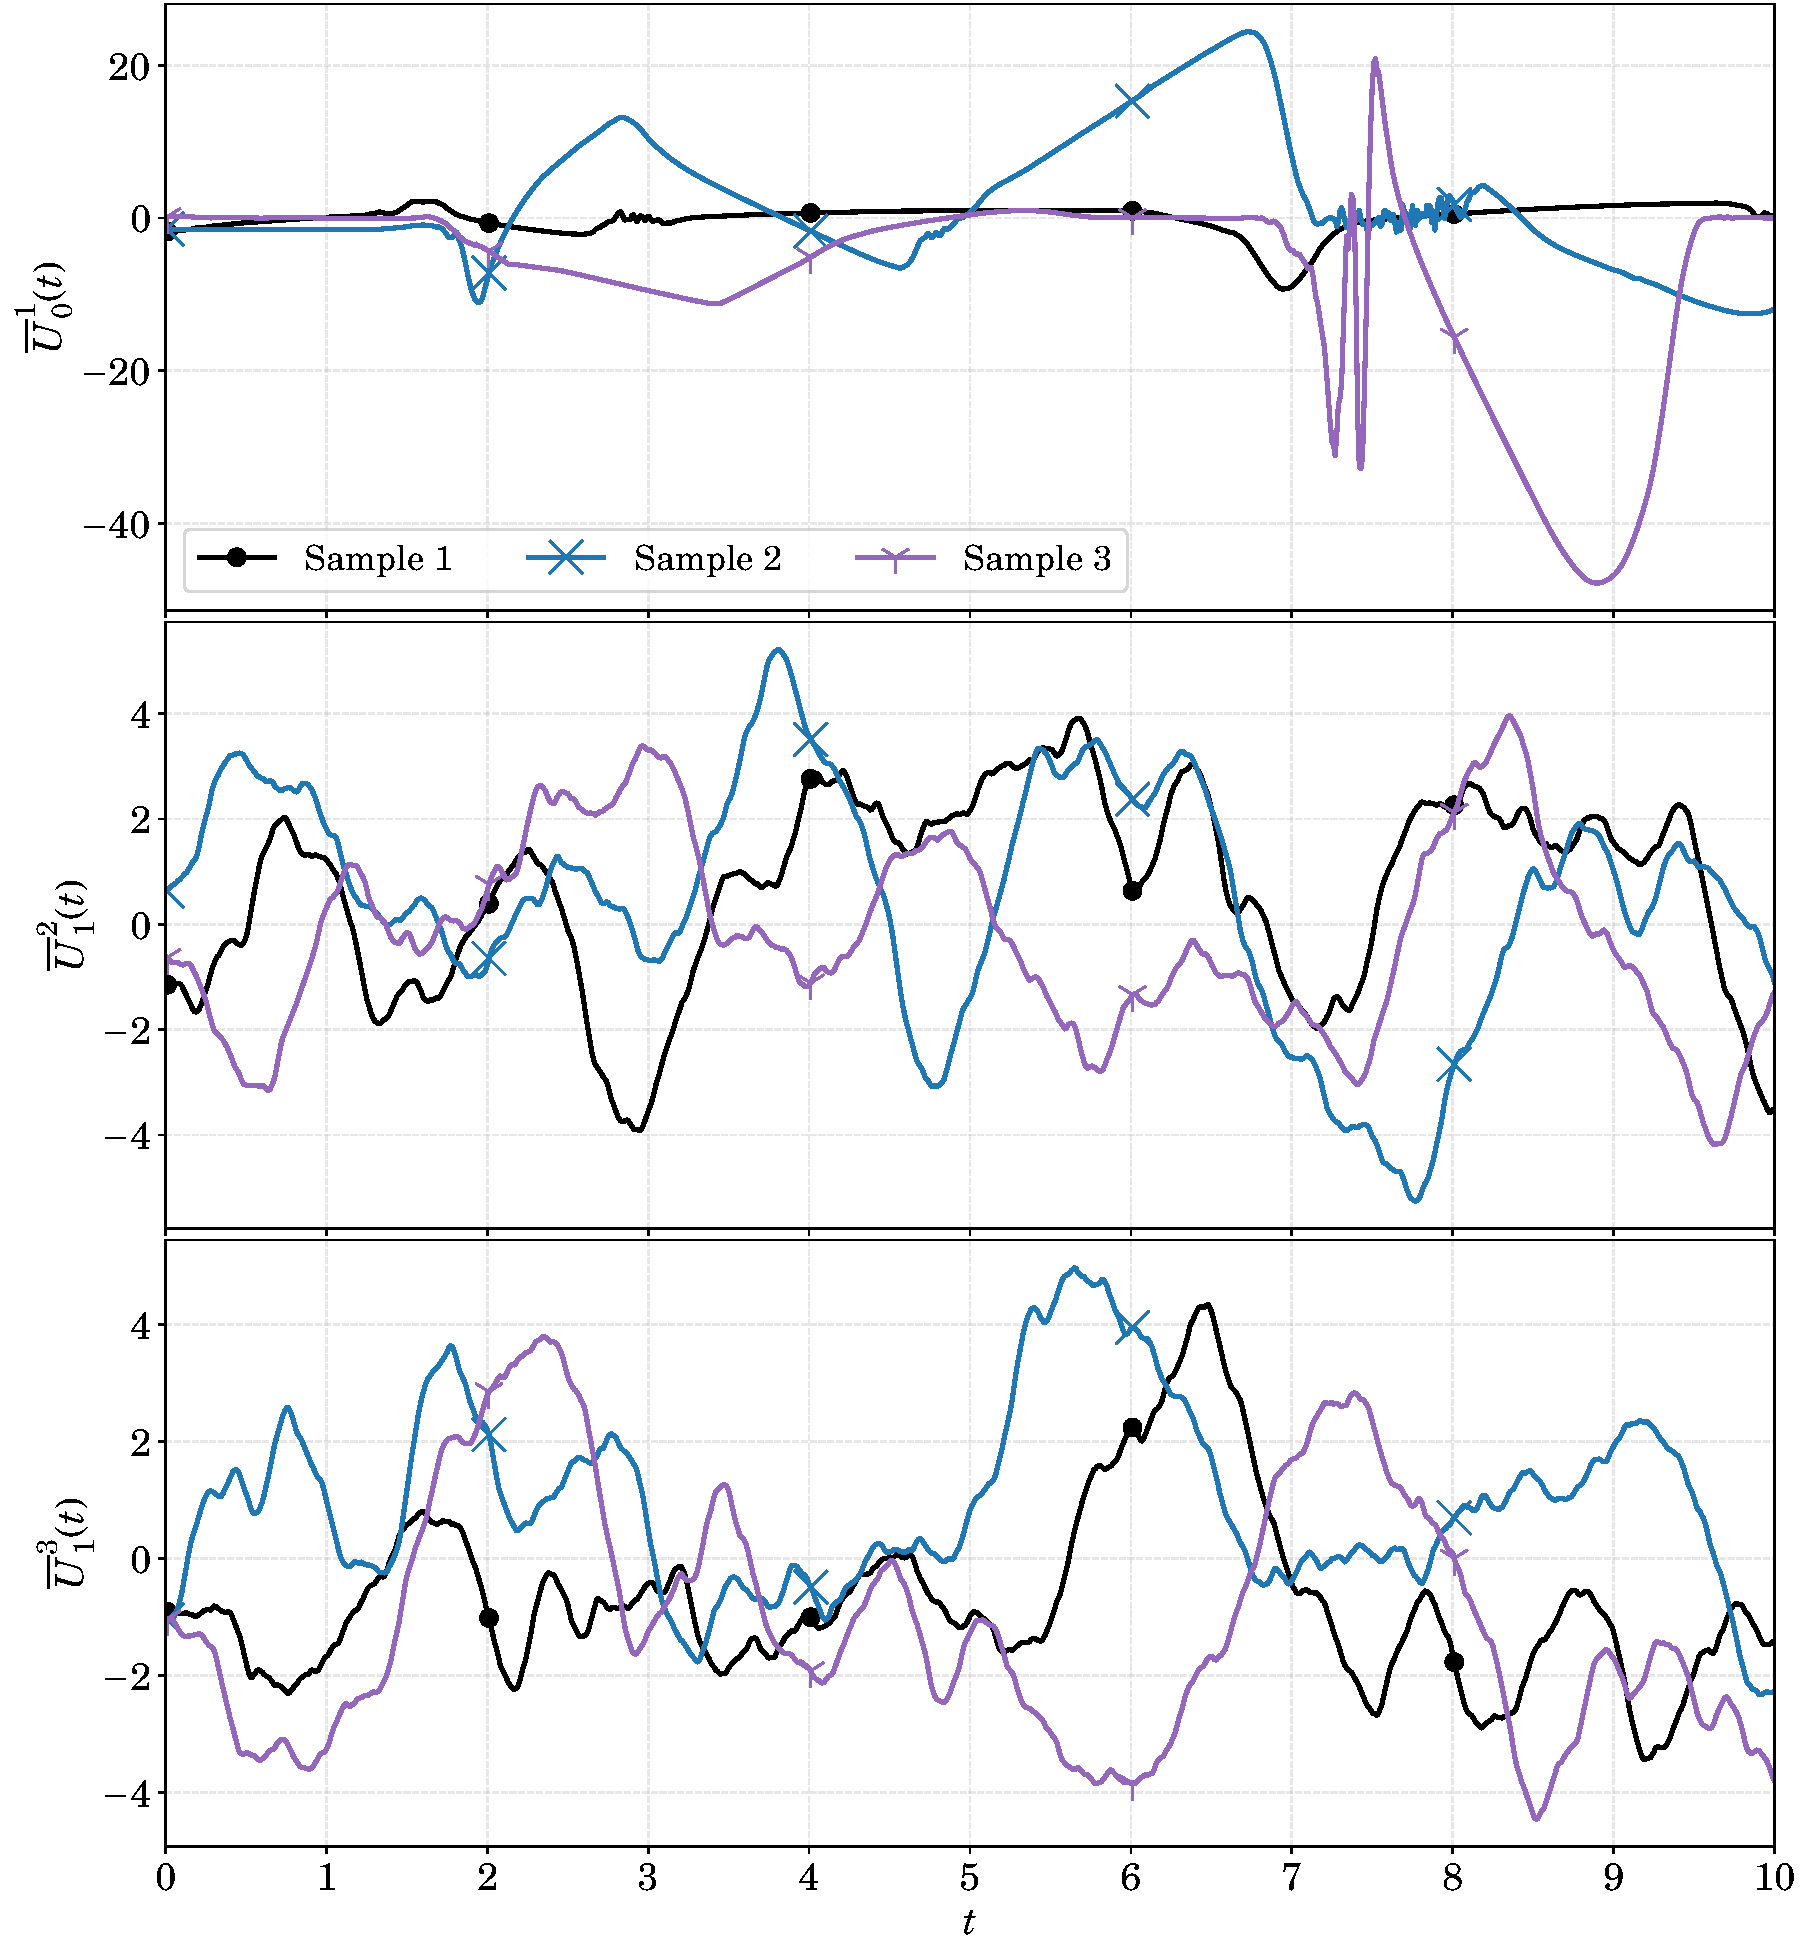
\includegraphics[width=\linewidth]{../thesis_latex/figs/samples_ssdgp_m32}
		\end{minipage}
		\begin{minipage}[c]{.32\linewidth}
			\caption{SS-DGP samples.}
		\end{minipage}
	\end{figure}
\end{frame}

\begin{frame}{SS-DGPs}
	\begin{figure}
		\begin{minipage}[c]{.62\linewidth}
			\centering
			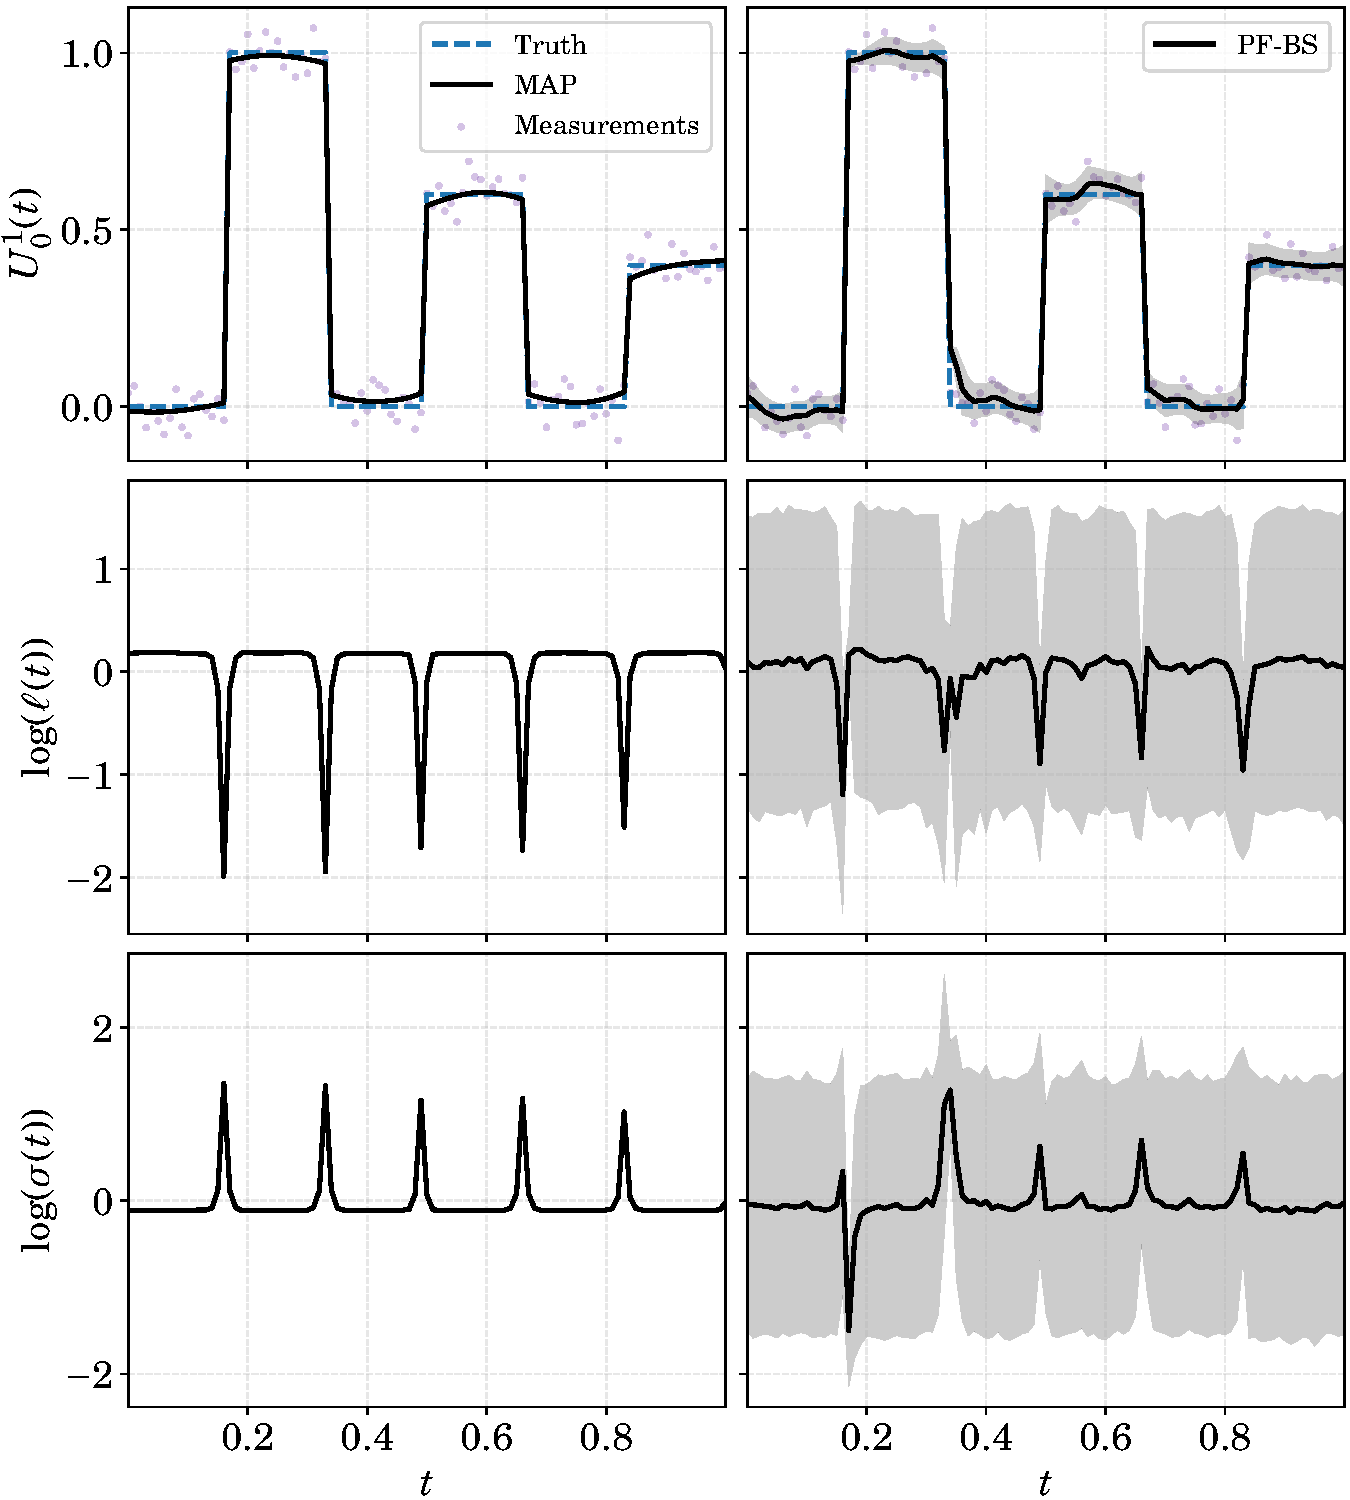
\includegraphics[width=\linewidth]{../thesis_latex/figs/ssdgp-reg-rect}
		\end{minipage}
		\begin{minipage}[c]{.37\linewidth}
			\caption{SS-DGP regression.}
		\end{minipage}
	\end{figure}
\end{frame}

\begin{frame}{}
	\begin{figure}
		\centering
		\begin{minipage}[c]{.62\linewidth}
			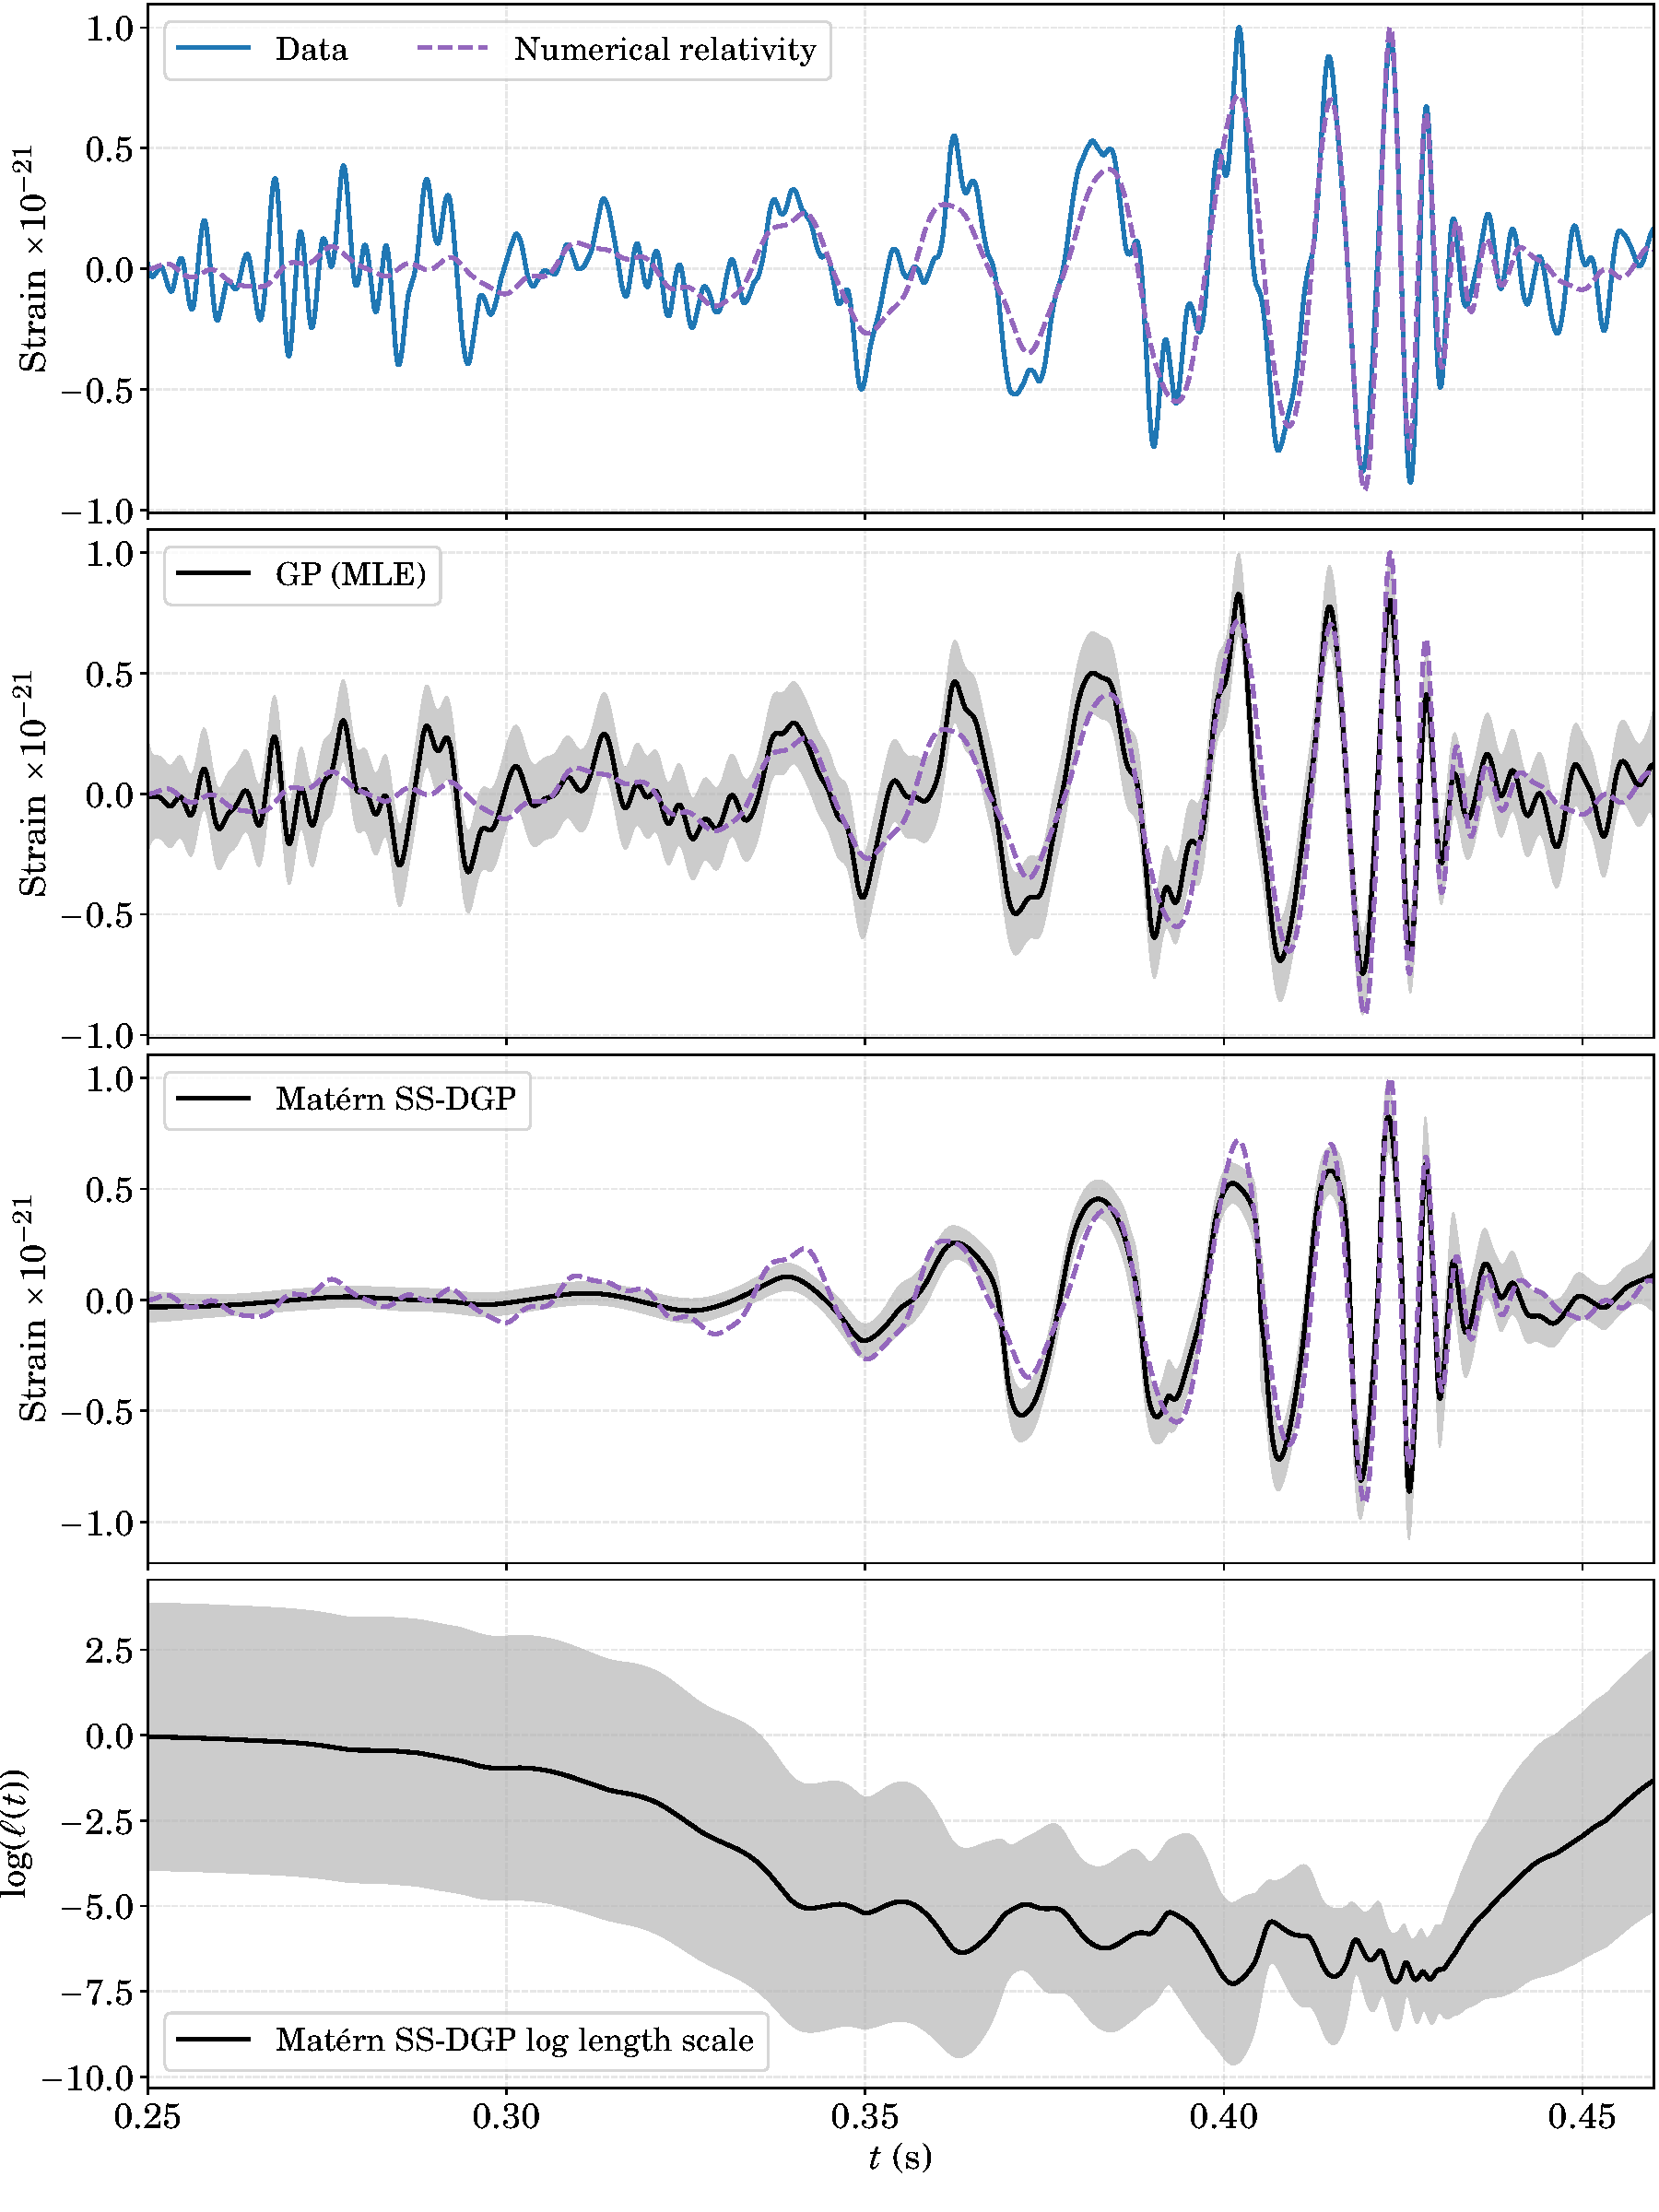
\includegraphics[width=\linewidth]{../thesis_latex/figs/gravit-wave-ssdgp}
		\end{minipage}
		\begin{minipage}[c]{.37\linewidth}
			\caption{Modelling gravitational wave with an SS-DGP.}
		\end{minipage}
	\end{figure}
\end{frame}

%\begin{frame}{SS-DGPs}
%	\begin{block}{}
%		However, there is an \alert{identifiability issue} if you solve SS-DGP regression using \alert{Gaussian filters and smoothers}. 
%	\end{block}
%	\begin{block}{}
%		For instance, suppose that 
%		%
%		\begin{equation}
%			\begin{split}
%				U(t) &\sim \GP(0, C(t, t'; \ell, \sigma)),\\
%				Y_k &= H \, U(t_k) + \xi_k,\\
%				g^{-1}(\sigma(t)) &\sim \GP(0, C_2(t, t')),\\
%				g &\colon \R\to\R_{>0},
%			\end{split}
%		\end{equation}
%		%
%		then it is \alert{hard} for Gaussian filters and smoothers to estimate the posterior distribution of $\sigma$ from data.
%	\end{block}
%	\begin{block}{}
%		The \alert{Kalman gain} for $\sigma$ converges to zero as $k\to\infty$.
%	\end{block}
%	\begin{block}{}
%		These are detailed in \alert{Section 4.8}.
%	\end{block}
%\end{frame}

\section{Applications of state-space (deep) Gaussian processes}
\begin{frame}{Contents}
	\begin{block}{}
		\tableofcontents[currentsection]
	\end{block}
\end{frame}

\begin{frame}{Probabilistic Drift Estimation}
	\begin{block}{}
		Consider an SDE
		%
		\begin{equation}
			\diff X(t) = a(X(t)) \diff t + b \diff W(t), \quad X(t_0) = X_0,
		\end{equation}
		%
		where the drift function $a$ is \alert{unknown}. The task is to estimate $a$ from a set of partial observations \alert{$x(t_1), x(t_2), \ldots, x(t_T)$} of the SDE.
	\end{block}
	\begin{block}{}
		One can assume that
		%
		\begin{equation}
			a(x) \sim \mathrm{SSGP}(0, C(x, x'))
		\end{equation}
		%
		then build an \alert{approximate likelihood} model from any \alert{discretisation} of the SDE.
	\end{block}
	\begin{block}{}
		If necessary, let $a$ follow an SS-DGP.
	\end{block}
\end{frame}

\begin{frame}{Probabilistic Drift Estimation}
	\begin{block}{}
		Essentially, the estimation model reads
		%
		\begin{equation}
			\begin{split}
				a(x) &\sim \mathrm{SSGP}(0, C(x, x')),\\
				X(t_k) - X(t_{k-1}) &\approx f_{k-1}(X_{k-1}) + q_{k-1}(X_{k-1}),
			\end{split}
		\end{equation}
		%
		where $f_{k-1}$ and $q_{k-1}$ are some \alert{non-linear functions and random variables} of $a$ and its \alert{derivatives} (depending on the discretisation).
	\end{block}
	\begin{block}{}
		What are the \alert{upsides} for placing an SS-(D)GP prior on $a$?
		\begin{itemize}
			\item \alert{Linear} time computational complexity.
			\item Derivatives of $a$ appear as \alert{state components}, no need to compute the covariance matrices of derivatives.
			\item Amenable to \alert{high-order discretisation schemes/accurate likelihood approxiamation}.
		\end{itemize}
	\end{block}
\end{frame}

%\begin{frame}{}
%	\begin{figure}
%		\centering
%		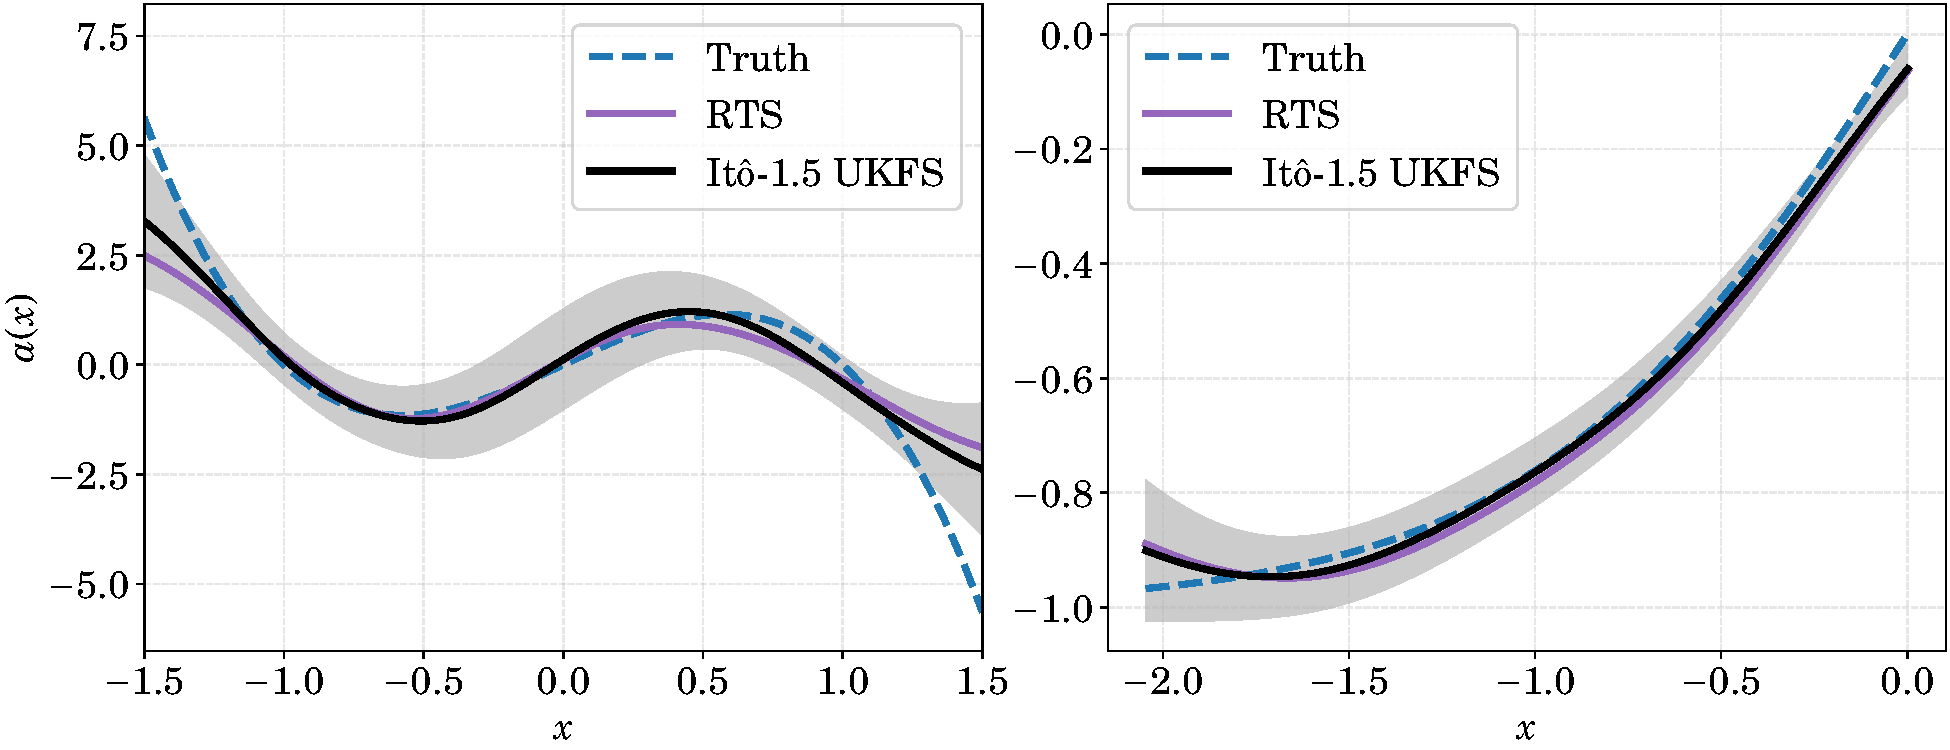
\includegraphics[width=\linewidth]{../thesis_latex/figs/drift-est}
%		\caption{Left: $a(x) = 3 \, (x-x^3)$. Right: $a(x) = \tanh(x)$.}
%	\end{figure}
%\end{frame}

\begin{frame}{Spectro-temporal Analysis}
	\begin{block}{}
		Consider any periodic signal $z\colon\T\to\R$. We may want to approximate it by \alert{Fourier expansion}:
		%
		\begin{equation}
			z(t) \approx \alpha_0 + \sum^N_{n=1} \big[ \alpha_n \cos(2 \, \pi \, f_n \, t) + \beta_n\sin(2 \, \pi \, f_n \, t) \big].
		\end{equation}
		%
		\alert{GP estimation} of the coefficients \alert{$\lbrace \alpha_0, \alpha_n,\beta_n \rbrace_{n=1}^N$}:
		%
		\begin{equation}
		\begin{split}
		\alpha_0(t) &\sim \mathrm{SSGP}(0, C^0_\alpha(t, t')), \\
		\alpha_n(t) &\sim \mathrm{SSGP}(0, C^n_\alpha(t, t')), \\
		\beta_n(t) &\sim \mathrm{SSGP}(0, C^n_\beta(t, t')), \\
		Y_k \alert{=} \alpha_0(t_k) + \sum^N_{n=1} \big[ \alpha_n(t_k) &\cos(2 \, \pi \, f_n \, t_k) + \beta_n(t_k)\sin(2 \, \pi \, f_n \, t_k) \big] + \xi_k,\nonumber
		\end{split}
		\end{equation}
	\end{block}
\end{frame}

\begin{frame}{Spectro-temporal Analysis}
	\begin{block}{}
		However, the approach is \alert{computationally demanding}. Needs to store and compute \alert{$2 \, N+1$} covariance matrices of dimension \alert{$T\times T$} and their \alert{inverse}.
	\end{block}
	\begin{block}{}
		If we use the state-space approach, then it reduces to solve \alert{$T$} covariance matrices of dimension \alert{$2 \, N+1$}. Beneficial when \alert{$T\gg N$}.
	\end{block}
	\begin{block}{}
		With a clever choice of \alert{stationary} state-space prior, the said covariance matrices are no longer a problem. Replaced by a \alert{pre-computed and data-independent} stationary covariance matrix. Even faster.
	\end{block}
	\begin{block}{}
		Detailed in \alert{Section 5.2}.
	\end{block}
\end{frame}

%\begin{frame}{}
%	\begin{figure}
%		\centering
%		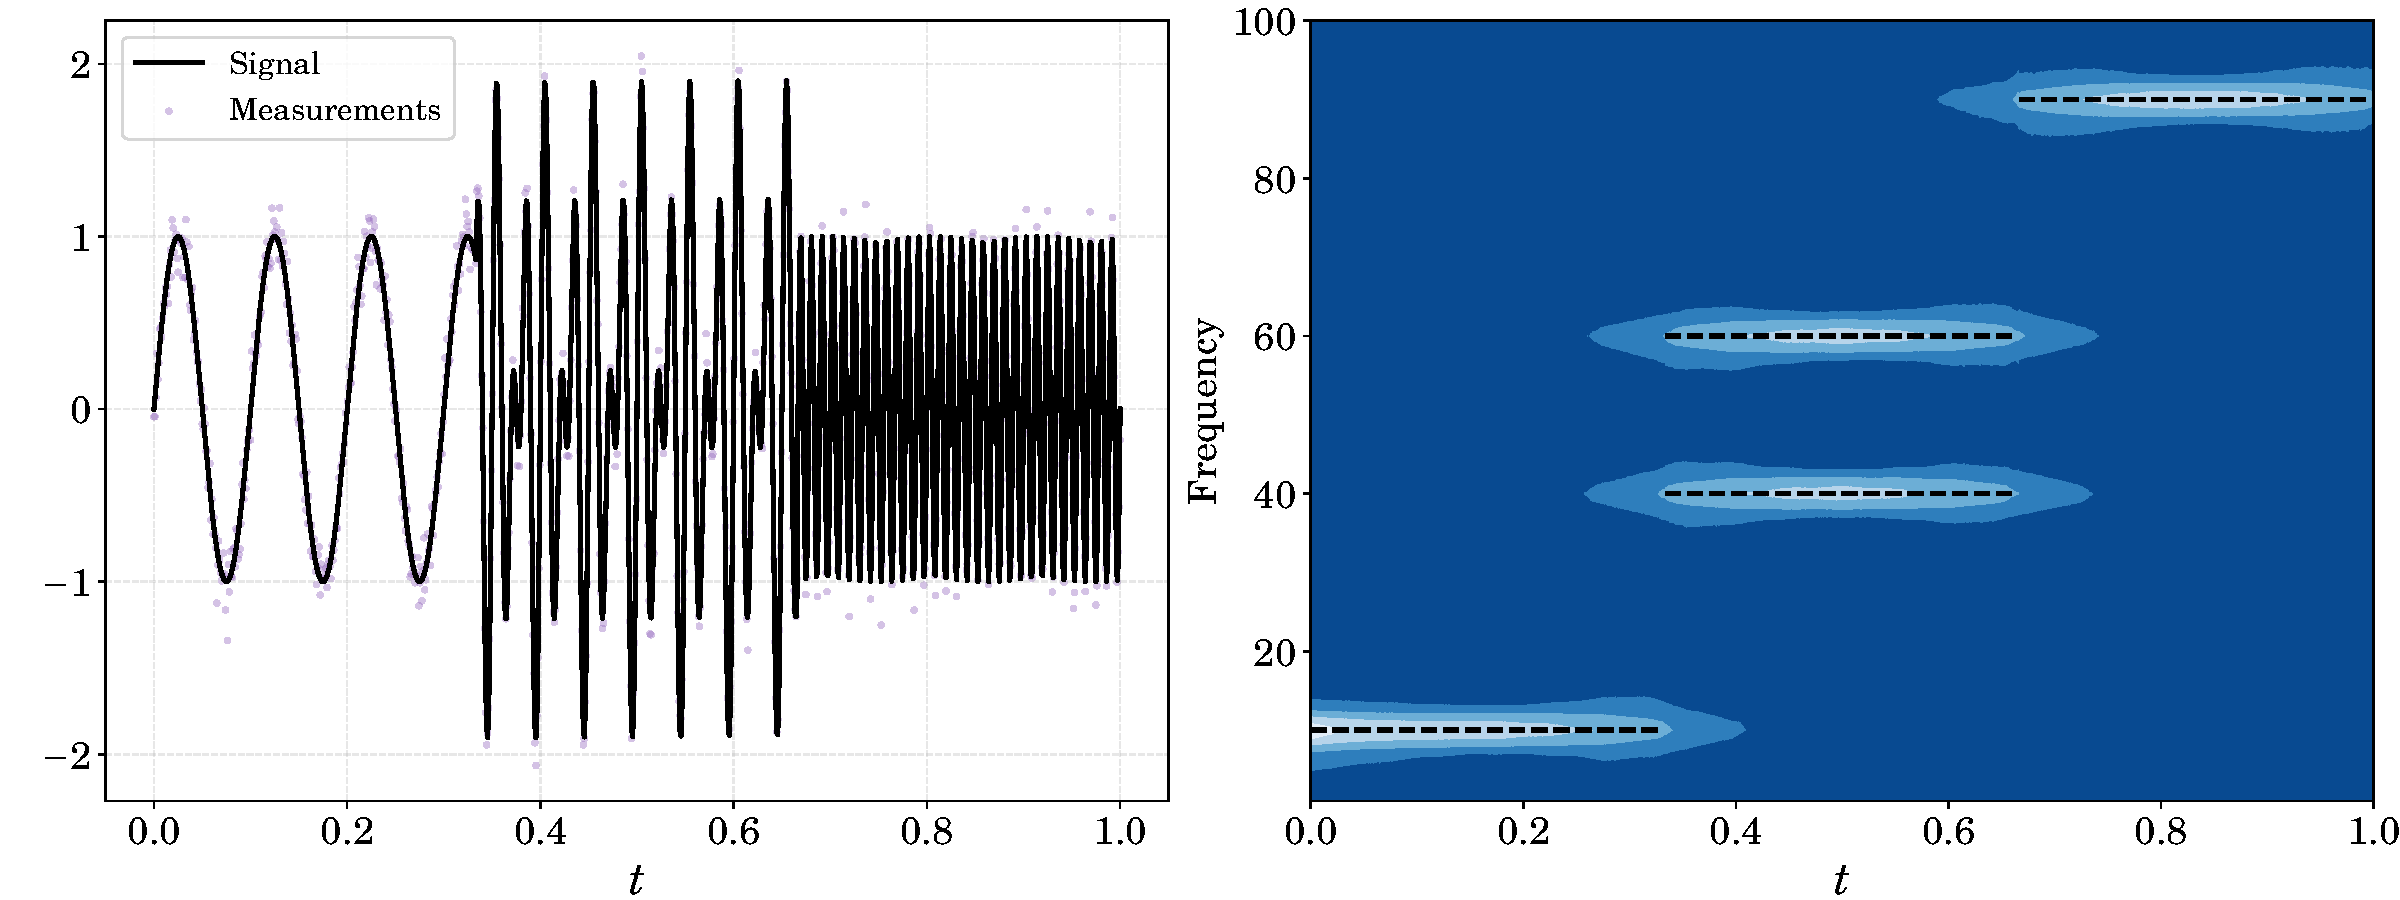
\includegraphics[width=\linewidth]{../thesis_latex/figs/spectro-temporal-demo1}
%		\caption{Spectrogram (right, contour plot) of a sinusoidal signal (left) estimated by RTS smoother. Dashed black lines stand for the ground truth frequencies.}
%	\end{figure}
%\end{frame}

\begin{frame}
	\noindent
	\begin{minipage}{.48\textwidth}
		\begin{figure}
			\centering
			\fbox{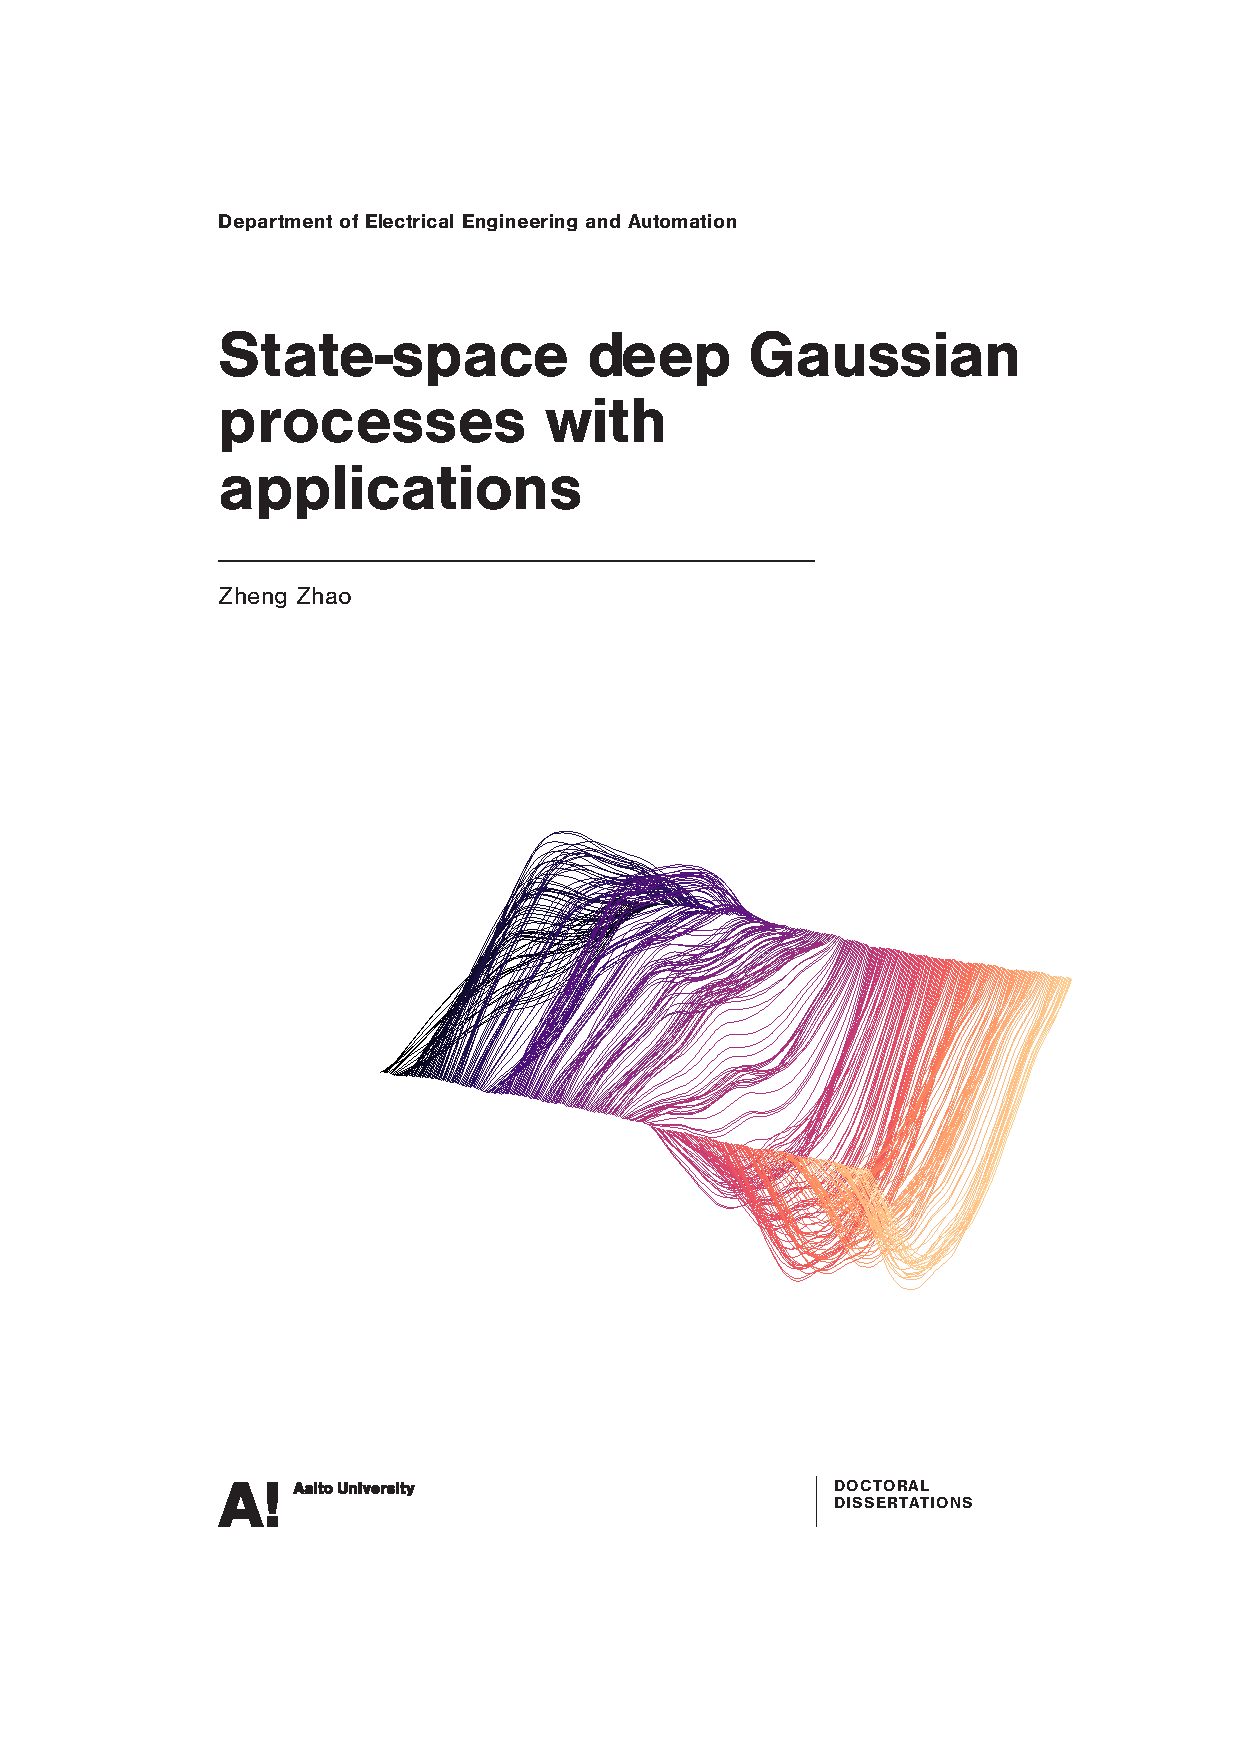
\includegraphics[trim={2cm 2cm 2cm 2cm},width=.8\linewidth,clip]{../thesis_latex/title-pages/title-pages}}
		\end{figure}
	\end{minipage}
	\hfill
	\begin{minipage}{.48\textwidth}
		\begin{block}{}
			Thank you!
		\end{block}
		\begin{block}{}
			\begin{figure}
				\centering
				
\includegraphics[width=.5\linewidth]{figs/qr-code-thesis}
			\end{figure}
		\end{block}
	\end{minipage}
\end{frame}

\end{document}